% http://www.idsc.ethz.ch/education/theses-semester-projects.html
% IDSC LaTeX Thesis Template
% 
% Author(s):	Eric Müller
% 				Institute for Dynamic Systems and Control
% 				Swiss Federal Institute of Technology (ETH) Zurich
% 
% Created:		2004/04/02  (Eric Mueller)
% 
% Notes: Has been tested on Windows 7 + MikTeX + TeXnicCenter
%
% Revisions: 	2009/05/29  (Soren Ebbesen)
% 				    2011/03/22	(Soren Ebbesen)
%             2013/03/08	(Soren Ebbesen)
%             2014/03/13	(Soren Ebbesen)
% ______________________________________________________________________________
\documentclass[10pt,twoside,a4paper]{report}

\usepackage{cite}
\usepackage{amsmath,amssymb,amsfonts}
\usepackage{mathrsfs}
\usepackage{algorithmic}
\usepackage{graphicx}
\usepackage{textcomp}
\usepackage{xcolor}
\usepackage{physics}
\usepackage{mathtools}
\usepackage{bbold}
\usepackage{lipsum}
\usepackage{enumitem}
\usepackage{parskip}
\usepackage{caption}
\usepackage{siunitx}
% \usepackage[retainorgcmds]{IEEEtrantools}

\setlist{nosep} % set itemized list style
\usepackage[english,mt]{ethidsc} % Special IDSC styles and commands      	
								 % {german}/english: language of headings, etc.
								 % {st}/bt/mt: {semester}/bachelor/master thesis
\usepackage{hyperref}
\usepackage[capitalise]{cleveref} % load cleverref as the last package!
\usepackage{crossreftools} % but load crossreftools after cleverref!

% \crefname{opt}{optimization problem}{optimization problems}
% \Crefname{opt}{Optimization problem}{Optimization problems}

\DeclarePairedDelimiter{\ceil}{\lceil}{\rceil}
\def\BibTeX{{\rm B\kern-.05em{\sc i\kern-.025em b}\kern-.08em
	T\kern-.1667em\lower.7ex\hbox{E}\kern-.125emX}}


% \renewcommand{\labelitemi}{\normalfont\bfseries\textendash}

\def\imagedir{img}

\theoremstyle{definition}
	\newtheorem{definition}{Definition}
	\newtheorem{assumption}{Assumption}
\theoremstyle{plain}
	\newtheorem{theorem}{Theorem}
	\newtheorem{lemma}{Lemma}
	\newtheorem{proposition}{Proposition}
\theoremstyle{remark}
	\newtheorem{remark}{Remark}

% redefine the reference styles
\crefname{equation}{}{}
\Crefname{equation}{}{}
% \crefname{definition}{Definition}{Definitions}
% \crefname{lemma}{Lemma}{Lemmas}
% \crefname{theorem}{Theorem}{Theorems}
% \crefname{remark}{Remark}{Remarks}
% \crefname{chapter}{Chapter}{Chapters}
% \crefname{section}{Section}{Sections}

% create new label for types of proofs
\newcounter{theoremproofcntr}
\newcounter{lemmaproofcntr}
\newcounter{propositionproofcntr}
\crefname{theoremproofcntr}{proof of Theorem}{proofs of Theorems}
\Crefname{theoremproofcntr}{Proof of Theorem}{Proofs of Theorems}
\crefname{lemmaproofcntr}{proof of Lemma}{proofs of Lemmas}
\Crefname{lemmaproofcntr}{proof of Lemma}{proofs of Lemmas}
\crefname{propositionproofcntr}{proof of Proposition}{proofs of Propositions}
\Crefname{propositionproofcntr}{proof of Proposition}{proofs of Propositions}

\NewDocumentCommand{\prooflabel}{o +m+m}{
	\setcounter{#1proofcntr}{\crtcrefcountervalue{#2}-1}
	\refstepcounter{#1proofcntr}
	% \crefformat{#1proofcntr}{#2\arabic{chapter}.#1#3}
	\label{#3}
	% \crtprovidecurrentlabel{\crtextractcref{reference}{#2}}
	% \crtprovidecurrentlabelname{#3}
}

\newcommand\includefig[4]{
	\begin{figure}[ht]
		\centering
		\includegraphics[width=#2\textwidth]{\imagedir/#1}
		\caption{#3}
		\label{#4}
	\end{figure}
}

\newcommand\defeq{\vcentcolon=}

\newcommand\tildex{\tilde{x}}
\newcommand\tildeu{\tilde{u}}
\newcommand\tildey{\tilde{y}}
\newcommand\hatx{\hat{x}}
\newcommand\hatu{\hat{u}}
\newcommand\haty{\hat{y}}
\newcommand\barx{\bar{x}}
\newcommand\baru{\bar{u}}
\newcommand\bary{\bar{y}}
\newcommand\starx{{x^*}}
\newcommand\staru{{u^*}}
\newcommand\stary{{y^*}}
\newcommand\checku{\check{u}}
\newcommand\checky{\check{y}}
\newcommand\checkx{\check{x}}

\newcommand\tildexi{\tilde{\xi}}
\newcommand\hatxi{\hat{\xi}}
\newcommand\barxi{\bar{\xi}}
\newcommand\starxi{{\xi^*}}

\newcommand\barvareps{\bar{\varepsilon}}
\newcommand\varepsmax{\varepsilon_{\text{max}}}

\newcommand\barD{\bar{D}}

\newcommand\us{{u^s}}
\newcommand\ys{{y^s}}
\newcommand\xs{{x^s}}

\newcommand\ud{{u^d}}
\newcommand\yd{{y^d}}

\newcommand\NH{{N_H}}

\newcommand\xelone{{x^{\scriptscriptstyle{(1)}}}}
\newcommand\xeltwo{{x^{\scriptscriptstyle{(2)}}}}

\newcommand\uObj{u^{\text{obj}}}

\newcommand\dataset{\mathcal{D}}

\newcommand\lamalpha{\lambda_\alpha}
\newcommand\lamsigma{\lambda_\sigma}

\newcommand\Up{{U_p}}
\newcommand\Uf{{U_f}}
\newcommand\Yp{{Y_p}}
\newcommand\tildeYp{{\tilde{Y}_p}}
\newcommand\Yf{Y_f}
\newcommand\tildeYf{{\tilde{Y}_f}}
\newcommand\hankeluy{
	\begin{bmatrix}
		\Up \\
		\Uf \\
		\Yp \\
	\end{bmatrix}
}
\newcommand\hankeluyone{
	\begin{bmatrix}
		\Up \\
		\Uf \\
		\Yp \\
		\transpose{\ones{\NH}}
	\end{bmatrix}
}
\newcommand\hankeluxone{
	\begin{bmatrix}
		\Uf \\
		\Yp \\
		\transpose{\ones{\NH}}
	\end{bmatrix}
}
\newcommand\hankelutildey{
	\begin{bmatrix}
		\Up \\
		\Uf \\
		\tildeYp \\
	\end{bmatrix}
}
\newcommand\hankelutildeyone{
	\begin{bmatrix}
		\Up \\
		\Uf \\
		\tildeYp \\
		\transpose{\ones{\NH}}
	\end{bmatrix}
}
\newcommand\Wt{{W_t}}
\newcommand\Dt{{D_t}}

\newcommand\rhoLmax{\rho_{L}^{\text{max}}}

\newcommand\infnorm[1]{\norm{#1}_\infty}
\newcommand\twonorm[1]{\norm{#1}_2}
\newcommand\onenorm[1]{\norm{#1}_1}

\newcommand\transpose[1]{#1^{\top}}
\newcommand\inv[1]{#1^{-1}}

\newcommand\mnormsq[2]{\transpose{#1} #2 #1}

\newcommand\ones[1]{\mathbb{1}_{#1}}
\newcommand\vRepeatVec[2]{\ones{#2} \otimes #1}

\newcommand\Real{\mathbb{R}}
\newcommand\Xset{\mathcal{X}}
\newcommand\Uset{\mathcal{U}}
\newcommand\Yset{\mathcal{Y}}
\newcommand\Sset{\mathcal{S}}
\newcommand\Epset{\mathcal{\Epsilon}}

\newcommand\RealVec[1]{\Real^{#1}}
\newcommand\RealMat[2]{\Real^{#1 \times #2}}

\newcommand\listinI[2]{\mathbb{I}_{\left[ #1, #2 \right]}}
\newcommand\sequence[4]{\left\{#1_#2\right\}_{#2=#3}^{#4}}
\newcommand\subseq[3]{#1_{\left[ #2, #3 \right]}}
\newcommand\hankel[2]{H_{#1}\left( #2 \right)}

\newcommand\datasetSequence[2]{\sequence{#1^d}{k}{0}{#2-1}}
\newcommand\constantSequence[3]{\sequence{#1}{k}{#2}{#3-1}}

							
% Page header (don't change)____________________________________________________
\setlength{\parindent}{0em}                 % Disable parindent
\rhead[\nouppercase{\rightmark}]{\thepage}  % Special headings
\lhead[\thepage]{\nouppercase{\leftmark}}   % Special headings
\cfoot{}                                    % Special headings


% Title page (please fill in)___________________________________________________
\title{Data-drive Predictive Safety Filter}


\studentA{Yujun Huang}
\ethidA{21-947-189}
\semesterA{4}
\emailA{yujhuang@student.ethz.ch}

%\studentB{Second Student}
%\ethidB{12-345-678}
%\semesterB{9}
%\emailB{second@student.ethz.ch}

\supervision{
    Dr. Andrea Carron \\
    Alexandre Didier \\
    Dr. Anna Scampicchio \\
    Prof. Dr. Melanie Zeilinger
}
\date{October 2023}

\identification{IDSC-AC-AD-AS-01} 		% Project identifier

\infopage
\declaration

% Begin document________________________________________________________________
\begin{document}

\maketitle 							% Create title page


% Preamble______________________________________________________________________

\pagenumbering{roman} 				% Begin roman page numbering (i,ii,...)

%---------------------------------------------------------------------------
% Preface

\chapter*{Preface}

Blah blah \dots

 \cleardoublepage

%---------------------------------------------------------------------------
% Table of contents

 \setcounter{tocdepth}{2}
 \tableofcontents

 \cleardoublepage

%---------------------------------------------------------------------------
% Abstract

\chapter*{Abstract}
 \addcontentsline{toc}{chapter}{Abstract}

In this thesis, we investigated the designing, analysis, and application of a novel data-driven predictive safety filter.
% Predictive safety filters can keep the system safe under arbitrary given control input, by predicting future states of the system and applying a safe input that is close to the given input.
The offline design of data-driven safety filters requires no knowledge of dynamics of the system, only some rich enough dataset trajectories of the system are needed.

For noise-free Linear Time Invariant (LTI) system, the data-driven safety filter is equivalent to the model-based safety filter.
The filter is also robust with respect to bounded noise.
In this case, qualitative guarantees can be given for the safety filter, including recursive feasibility and constraint satisfaction in close loop.

For general non-linear system, the safety filter can also perform well in practice.
We propose a method of improving the performance by selecting and putting different weights on trajectory slices.
It is tested on the kinematic and dynamic model of Chronos vehicle.
It can be seen that the safety filter can keep the vehicle within the given safe constraints, while keeping the actual input as close as possible to the desired input.

Question: add description and introduction to each chapter?

 \cleardoublepage

%---------------------------------------------------------------------------
% Symbols

\chapter*{Nomenclature}\label{chap:symbole}
 \addcontentsline{toc}{chapter}{Nomenclature}

\section*{Symbols}
\begin{tabbing}
 \hspace*{1.6cm} \= \hspace*{8cm} \= \kill
 $\mathrm{EHC}$ \> Conditional equation \> [$-$] \\[0.5ex]
 $e$ \> Willans coefficient \> [$-$] \\[0.5ex]
 $F,G$ \> Parts of the system equation \> [\unitfrac[]{K}{s}]
\end{tabbing}

\section*{Indicies}
\begin{tabbing}
 \hspace*{1.6cm}  \= \kill
 a \> Ambient \\[0.5ex]
 air \> Air
\end{tabbing}

\section*{Acronyms and Abbreviations}
\begin{tabbing}
 \hspace*{1.6cm}  \= \kill
 NEDC \> New European Driving Cycle \\[0.5ex]
 ETH \> Eidgen\"{o}ssische Technische Hochschule
\end{tabbing}

 \cleardoublepage

%---------------------------------------------------------------------------


% Chapters______________________________________________________________________

\pagestyle{fancy}               	% Fancy headings
\pagenumbering{arabic}				% Begin arabic page numbering (1,2,...)

\chapter{Introduction}\label{chap:introduction}
TODO: Contains introduction, motivation, background, literature review, and outline of the thesis.

\begin{lemma}\label{lemma:fundamental-lemma}
    If dataset trajectory rich enough, and the LTI system is controllable, then...
\end{lemma}

We have the model-based safety filter as:
\begin{IEEEeqnarray}{RL}\label{eq:model-based-safety-filter}
    \min_{\substack{\bar{u}, \bar{y} \\ \bar{x}}} \quad & \norm{u_{[0]} - u^{\text{obj}}}_R^2 \IEEEyesnumber \IEEEyessubnumber* \label{model-based-safety-filter-cost}\\
    \textrm{s.t.} \quad & 
    \bar{x}_{k+1} = A \bar{x}_k + B \bar{u}_k \IEEEnonumber \\
    &
    \bar{y}_k = C \bar{x}_k + D \bar{u}_k,  \quad k \in \left[-n, L-1\right] \label{model-based-safety-filter-dynamics} \\
    & 
    \begin{bmatrix}
        \subseq{-n}{-1}{\bar{u}} \\
        \subseq{-n}{-1}{\bar{y}} \\
    \end{bmatrix} = 
    \begin{bmatrix}
        \subseq{t-n}{t-1}{u} \\
        \subseq{t-n}{t-1}{y} \\
    \end{bmatrix} \label{model-based-safety-filter-initial}\\
    & 
    \begin{bmatrix}
        \subseq{L-n}{L-1}{\bar{u}} \\
        \subseq{L-n}{L-1}{\bar{y}} \\
    \end{bmatrix} = 
    \begin{bmatrix}
        u_n^s \\
        y_n^s \\
    \end{bmatrix} \label{model-based-safety-filter-terminal}\\
    &
    \bar{u}_k \in \mathbb{U}, \quad k \in \left[0, L-1\right] \label{model-based-safety-filter-input}\\
    &
    \bar{y}_k \in \mathbb{Y}, \quad k \in \left[0, L-1\right] \label{model-based-safety-filter-output}
\end{IEEEeqnarray}

\cleardoublepage
\chapter{Nominal Data-Driven Safety Filter}\label{chap:nominal-ddsf}

In this chapter, we focus on the design of safety filters for noise-free LTI system.
We will first introduce the formulation of model-based safety filter and nominal data-driven safety filter, respectively.
Then we show that the nominal data-driven safety filter is equivalent to the model-based safety filter for noise-free LTI system.
Finally, we discuss the possible improvements on the designing of nominal data-driven safety filter.


\section{Model-Based and Data-Driven Safety Filter for LTI system}\label{sec:formulation-nominal}

As discussed in \cref{chap:introduction}, the predictive safety filter \cref{eq:state-based-safety-filter} is designed based on the assumption that the system state is fully observable.
Since we are working with noise-free LTI system that only the output is observable, we need to reformulate the safety filter \cref{eq:state-based-safety-filter} to an output-based safety filter as follows:

\begin{subequations}
\label{eq:model-based-safety-filter}
\begin{align}
    \min_{\substack{\bar{u}, \bar{y} \\ \bar{x}}} \quad & \norm{\baru_{0} - u^{\text{obj}}}_R^2 \label{eq:model-based-safety-filter-cost} \\
    \textrm{s.t.} \quad & 
    \bar{x}_{k+1} = A \bar{x}_k + B \bar{u}_k \nonumber \\
    &
    \bar{y}_k = C \bar{x}_k + D \bar{u}_k,  \quad k \in \left[-n, L-1\right] \label{eq:model-based-safety-filter-dynamics} \\
    & 
    \begin{bmatrix}
        \subseq{\bar{u}}{-n}{-1} \\
        \subseq{\bar{y}}{-n}{-1} \\
    \end{bmatrix} = 
    \begin{bmatrix}
        \subseq{u}{t-n}{t-1} \\
        \subseq{y}{t-n}{t-1} \\
    \end{bmatrix} \label{eq:model-based-safety-filter-initial}\\
    & 
    \begin{bmatrix}
        \subseq{\bar{u}}{L-n}{L-1} \\
        \subseq{\bar{y}}{L-n}{L-1} \\
    \end{bmatrix} = \begin{bmatrix}
        \vRepeatVec{\us}{n} \\
        \vRepeatVec{\ys}{n} \\
    \end{bmatrix} \label{eq:model-based-safety-filter-terminal}\\
    &
    \bar{u}_k \in \Uset, \quad k \in \left[0, L-1\right] \label{eq:model-based-safety-filter-input}\\
    &
    \bar{y}_k \in \Yset, \quad k \in \left[0, L-1\right] \label{eq:model-based-safety-filter-output}
\end{align}
\end{subequations}

Where $\us$ and $\ys$ are a pair of safe input-output equilibrium, as defined in \cref{def:input-output-equilibrium} and \cref{remark:safe-equilibrium}.
It still follows the predictive safety filter idea: evaluate the safety of a proposed input sequence by predicting future trajectory of the system, and the objective \cref{eq:model-based-safety-filter-cost} is also designed to minimize the deviation from the given control input.
But there are some further discussions needed for this formulation:

\begin{enumerate}
    \item The optimization variables not only include candidate input sequence $\baru$ and output sequence $\bary$, but also the state sequence $\barx$.
    Since we are working with system dynamics, this is necessary.
    \item Since we only observe the output of the system, more than one step of input-output pairs are needed to uniquely determine the state of the system.
    This is reflected in \cref{eq:model-based-safety-filter-initial}.
    Here we choose to use the most recent $n$ steps of input-output pairs to uniquely determine the inner state of the system.
    \item The terminal constraint \cref{eq:model-based-safety-filter-terminal} is less general than \cref{eq:state-based-safety-filter-terminal}.
    As discussed in \cref{remark:safe-traj}, a long enough safe trajectory can be used to ensure the safety of system in all future time steps.
    Here we use a safe input-output equilibrium to construct such a safe trajectory.
    More complicated terminal constraints can be used, as will be briefly discussed in \cref{sec:improvements-nominal}.
    \item Due to the form of terminal condition \cref{eq:model-based-safety-filter-terminal}, the prediction horizon $L$ needs to be larger than $n$.
    In fact, since the last $n$ steps of input-output pairs are used to determine the terminal state $\xs$ at time step $L-n$, the actual prediction horizon (time steps before the system is constraint to be inside the terminal set) is $L-n$.
\end{enumerate}

This formulation also provides closed-loop guarantees similar to the state-based safety filter \cref{eq:state-based-safety-filter}.

\begin{theorem}[Closed-loop Guarantees for Model-based Safety Filter]\label{thm:guarantee-model-based-lti}
    When the system is equipped with the safety filter \cref{eq:model-based-safety-filter}, and a one-step receding horizon scheme, closed-loop constraint satisfaction and recursive feasibility hold.
\end{theorem}

\begin{proof}[Proof of \Cref{thm:guarantee-model-based-lti}]\prooflabel[theorem]{thm:guarantee-model-based-lti}{prf:guarantee-model-based-lti}
    First we show constraint satisfaction for the next time step, then we show recursive feasibility by providing a feasible solution for the next time step.
    Then the closed-loop constraint satisfaction for all future time steps is shown by induction.

    Due to initial constraint \cref{eq:model-based-safety-filter-initial} and dynamic constraint \cref{eq:model-based-safety-filter-dynamics}, the initial state of the system $x_t$ is the same as the optimal solution $\starx_0(t)$.
    Then due to dynamic constraint \cref{eq:model-based-safety-filter-dynamics}, after $\staru_0$ is applied to the real system, the output will be $\stary_0(t)$, which satisfies the constraint $\Yset$ due to \cref{eq:model-based-safety-filter-output}.

    At time step $t+1$, we define the candidate solution $\hatu(t+1)$, $\hatx(t+1)$, and $\haty(t+1)$ as follows:
    {
    \setlength{\abovedisplayskip}{3pt}
    \setlength{\belowdisplayskip}{3pt}
    % \setlength{\abovedisplayshortskip}{0pt}
    % \setlength{\belowdisplayshortskip}{0pt}
    \begin{align*}
        \subseq{\hatu}{-n}{L-2}(t+1) = \subseq{\staru}{-n+1}{L-1}(t), \quad \hatu_{L-1}(t+1) = \us \\
        \subseq{\hatx}{-n}{L-2}(t+1) = \subseq{\starx}{-n+1}{L-1}(t), \quad \hatx_{L-1}(t+1) = \xs \\
        \subseq{\haty}{-n}{L-2}(t+1) = \subseq{\stary}{-n+1}{L-1}(t), \quad \haty_{L-1}(t+1) = \ys
    \end{align*}
    }
    Where $\xs$ is the equilibrium state implicitly defined by $\us$ and $\ys$.
    Due to terminal constraint \cref{eq:model-based-safety-filter-terminal}, we have $\hatx_{L-2}(t+1) = \xs$, also because the optimal solution $\staru(t)$, $\starx(t)$, and $\stary(t)$ satisfy the dynamic constraint \cref{eq:model-based-safety-filter-dynamics}, we can conclude that $\subseq{\hatu}{-n}{L-1}(t+1)$, $\subseq{\hatx}{-n}{L-1}(+1)$, and $\subseq{\haty}{-n}{L-1}$ is a trajectory of the system, thus satisfies the dynamic constraint \cref{eq:model-based-safety-filter-dynamics}.

    It's also easy to verify that \crefrange{eq:model-based-safety-filter-initial}{eq:model-based-safety-filter-terminal} are also satisfied by the candidate solution.

    So recursive feasibility is shown.
\end{proof}

\begin{remark}\label{remark:usage-output-safety-filter}
    As seen in the formulation \cref{eq:model-based-safety-filter}, the safety filter needs more than one step of input-output pairs as the initial condition.
    This can be problematic at first time steps, when there are not enough input-output pairs available.
    To walk around this problem, we can either run the system without a safety filter for a few time steps, or use expert knowledge to construct a proper initial condition.
\end{remark}

Based \cref{lemma:fundamental-lemma}, the dataset trajectory can be used to reconstruct the system dynamic constraint in the model-based safety filter \cref{eq:model-based-safety-filter}.
So we can formulate the nominal data-driven safety filter as:

\begin{subequations}
\label{eq:nominal-ddsf} 
\begin{align}
    \min_{\alpha, \bar{u}, \bar{y}} \quad & \norm{\baru_{0} - u^{\text{obj}}}_R^2  \label{eq:nominal-ddsf-cost}\\
    \textrm{s.t.} \quad & 
    \begin{bmatrix}
        \subseq{\bar{u}}{-n}{L-1} \\
        \subseq{\bar{y}}{-n}{L-1} \\
    \end{bmatrix} = 
    \begin{bmatrix}
        \hankel{L+n}{u^d} \\
        \hankel{L+n}{y^d} \\
    \end{bmatrix} \alpha \label{eq:nominal-ddsf-dynamics}\\
    & 
    \begin{bmatrix}
        \subseq{\bar{u}}{-n}{-1} \\
        \subseq{\bar{y}}{-n}{-1} \\
    \end{bmatrix} = 
    \begin{bmatrix}
        \subseq{u}{t-n}{t-1} \\
        \subseq{y}{t-n}{t-1} \\
    \end{bmatrix} \label{eq:nominal-ddsf-initial}\\
    & 
    \begin{bmatrix}
        \subseq{\bar{u}}{L-n}{L-1} \\
        \subseq{\bar{y}}{L-n}{L-1} \\
    \end{bmatrix} = 
    \begin{bmatrix}
        u_n^s \\
        y_n^s \\
    \end{bmatrix} \label{eq:nominal-ddsf-terminal}\\
    &
    \bar{u}_k \in \Uset, \quad k \in \left[0, L-1\right] \label{eq:nominal-ddsf-input}\\
    &
    \bar{y}_k \in \Yset, \quad k \in \left[0, L-1\right] \label{eq:nominal-ddsf-output}
\end{align}
\end{subequations}

As described above, the constraint \cref{eq:nominal-ddsf-dynamics} replaces the system dynamic constraint \cref{eq:model-based-safety-filter-dynamics} in the model-based safety filter.
Where $u^d$ and $y^d$ represent a dataset trajectory of length $N$: $\datasetSequence{u}{N}$ and $\datasetSequence{y}{N}$.

And we have the following theorem:

\begin{theorem}[Equivalence of Data-driven and Model-based Safety Filters]\label{thm:nominal-equivalence}
    Suppose:
    \begin{enumerate}
        \item The system is a controllable LTI system.
        \item The dataset input sequence $\datasetSequence{u}{N}$ is persistently exciting with order $(L+n)+n$, where $L$ is the prediction horizon and $n$ is order of the system.
    \end{enumerate}
    Then we have: the optimization problem \cref{eq:nominal-ddsf} is equivalent to the optimization problem \cref{eq:model-based-safety-filter}.
    In another word, any feasible solution of \cref{eq:nominal-ddsf} can be transformed to a feasible solution of \cref{eq:model-based-safety-filter} with the same candidate input sequence, and vice versa.
\end{theorem}

\begin{proof}[Proof of \Cref{thm:nominal-equivalence}]\prooflabel[theorem]{thm:nominal-equivalence}{prf:nominal-equivalence}
    Since the constraints \crefrange{eq:model-based-safety-filter-initial}{eq:model-based-safety-filter-terminal} and \crefrange{eq:nominal-ddsf-initial}{eq:nominal-ddsf-terminal} are identical, we only need to show that the dynamic constraints \cref{eq:model-based-safety-filter-dynamics} and \cref{eq:nominal-ddsf-dynamics} can satisfied with the same candidate input sequence.

    First suppose $\baru_D$ and $\bary_D$ is a feasible solution of \cref{eq:nominal-ddsf}.
    Then by \cref{lemma:fundamental-lemma} and the conditions of \cref{thm:nominal-equivalence}, we can conclude that $\baru_D$ and $\bary_D$ form a trajectory of the system, of length $L+n$.
    Then we can define $\barx_D$ as the state sequence of the system corresponding to $\baru_D$ and $\bary_D$.
    Since $\baru_D$, $\barx_D$ and $\bary_D$ is a trajectory of the system, it satisfies the dynamic constraint \cref{eq:model-based-safety-filter-dynamics}.

    Then suppose $\baru_M$, $\barx_M$ and $\bary_M$ is a feasible solution of \cref{eq:model-based-safety-filter}.
    Then due to the dynamic constraint \cref{eq:model-based-safety-filter-dynamics}, $\baru_M$, $\barx_M$ and $\bary_M$ is a trajectory of the system, of length $L+n$.
    Again due to \cref{lemma:fundamental-lemma} and the conditions of \cref{thm:nominal-equivalence}, we can conclude that $\baru_M$ and $\bary_M$ is a feasible solution of \cref{eq:nominal-ddsf}, with proper choice of $\alpha$.
\end{proof}

Combining \cref{thm:guarantee-model-based-lti} and \cref{thm:nominal-equivalence}, we can conclude that the nominal data-driven safety filter \cref{eq:nominal-ddsf} also provides closed-loop guarantees for controllable LTI system.


\section{Improvements on Nominal Data-Driven Safety Filter}\label{sec:improvements-nominal}

For the nominal data-driven safety filter \cref{eq:nominal-ddsf}, the most important conservative comes from the terminal constraint \cref{eq:nominal-ddsf-terminal}.
Generally speaking, we only need the last $n$ steps of input-output pairs $\subseq{\baru}{L-n}{L-1}$ and $\subseq{\bary}{L-n}{L-1}$ to be a safe trajectory as defined in \cref{def:safe-traj}.
By the definition of safe trajectory, we can also use a proof similar to \cref{prf:guarantee-model-based-lti} to show that with this modification of terminal constraint, the safety filter \cref{eq:nominal-ddsf} still provides closed-loop guarantees for controllable LTI system.

However, it is generally difficult to find the set of all safe trajectories of length $n$ for a given system, even if the system is LTI and controllable.
It is easier and possible to find an \emph{Invariant Set} of the system instead, as discussed in \cite{berberichDesignTerminalIngredients2021}.
As discussed in \cite{berberichDesignTerminalIngredients2021}, the invariant set can be defined with respect to the \emph{extended state} of the system, which contains $n$ input-output pairs of the system.
The main drawback of this method includes: first it is required that $l \times p = n$; second it only provides method of estimating the invariant set form \emph{noise-free dataset}.

Further discussion about the invariant set in an input-output manner, as well as the possibility of using noisy dataset to estimate the invariant set, is left for future work.

As will be discussed in \cref{chap:test-chronos}, it's also possible to use expert knowledge about a certain system to design specific terminal constraint, which can be used to improve the performance of the safety filter.

\cleardoublepage
\chapter{Robust Data-Driven Safety Filter}\label{chap:robust-ddsf-lti}

In this chapter, we will discuss and compare different formulations of robust data-driven safety filters for LTI system with bounded output noise.
We will first introduce the direct formulation of the robust data-driven safety filter with rigorous constraint tightening scheme, and illustrate its limitations using a single-input-single-output (SISO) LTI system.
Then we will introduce the indirect formulation with qualitative constraint tightening scheme, and show that it can overcome the limitations of the direct formulation.

Before jumping into the details of data-driven safety filters, we first introduce the system we will be working with: LTI system with bounded output noise, as well as some notations that will be used later.

\begin{definition}[LTI System with Output Noise]\label{def:lit-output-noise}
    Starting from an LTI system without noise, as defined in \cref{def:dynamic-system} with linear dynamic and output functions, we can add a bounded output noise to the system.
    In another word, we can only observe $\tildey = y + \varepsilon$, where $\varepsilon$ is an unknown noise.

    We do not discuss or care about the distribution or stochastic properties of $\varepsilon$, the only condition we put on it is that it is bounded by a known constant $\barvareps$: $\infnorm{\varepsilon} \leq \barvareps$.
\end{definition}

\begin{remark}\label{remark:state-noise-lti}
    Although we do not explicitly deal with state noise in this chapter, we can incorporate bounded state noise when the system is \emph{asymptotically stable}.
    We do not discuss this point in detail in this Thesis.

    The intuition is, ``noise on the state'' will be transformed into ``noise on the output'' by the system dynamics.
    If the dynamics is asymptotically stable, this transformed noise on output will also be bounded.
\end{remark}

To simplify the discussion, we also assume the output constraint is a hypersquare, that is: $\Yset = \left\{y \, | \, \infnorm{y} \leq y_{\text{max}}\right\}$.

Within this chapter and the proof in appendix \cref{apps:prf-roubust-direct,apps:prf-roubust-indirect}, we will use the following notation:
Variables with tilde, like $\tildey$ represent observed variables with noise.
We will use $\varepsilon$ to represent noise variables, and $\barvareps$ to represent bound of the noise.
Note that usually we also extensively use variables with bar, like $\bary$, to represent the optimization variables.
This will not cause too much confusion, since noise variables are usually not optimization variables.

Also, similar to the notation in \cite{berberichDataDrivenRobust2021}, we use $\xi$ to denote the extended state of the system, which is a long vector that contains necessarily input-output pairs to determine the state of the system
For example, at time step $t$, the extended state can be written as $\xi_t = \transpose{\begin{bmatrix} \transpose{\subseq{u}{t-n}{t-1}} & \transpose{\subseq{y}{t-n}{t-1}} \end{bmatrix}}$.
Similar to other variables, it also has the version with output noise: $\tildexi_t = \transpose{\begin{bmatrix} \transpose{\subseq{u}{t-n}{t-1}} & \transpose{\subseq{\tildey}{t-n}{t-1}} \end{bmatrix}}$.
Note that we do not consider input noise in this Thesis, so the input is always exact.
Depending on the context, the number of input-output pairs used to construct $\xi$ can be $l$ or $n$.


\section{Direct Formulation}\label{sec:direct-formulation}

As has been discussed in \cite{coulsonDataenabledPredictiveControl2019}, when the dataset output sequence $\datasetSequence{\tildey}{N}$ is noisy, the Hankel matrix $\hankel{L+n}{\tildey^d}$ will become full rank, which means the column space of $\hankel{L+n}{\tildey^d}$ will be $\Real^{m(L+n)}$.
In another word, the original data driven safety filter formulation \cref{eq:nominal-ddsf} will be able to make \emph{any prediction} possible.

To overcome this problem, it is advised in \cite{coulsonDataenabledPredictiveControl2019} to add a regularizer into the objective function.
As mentioned in \cref{sec:motivation-and-background}, we have a lot of discussions about choices and properties of different regularizers.
To allow more discussion about guarantees, we will use a \emph{2-norm} regularizer.

Also, as in common MPC schemes, it is also necessary to modify the constraint to deal with the noise.
We incorporate the constraint tightening scheme proposed and analysed in \cite{berberichRobustConstraintSatisfaction2020}.

The final point mention here is, we will consider the n-step receding horizon scheme, in contrast to the one-step receding horizon scheme used for nominal data-driven safety filter introduced in \cref{chap:nominal-ddsf}. 
Namely, the optimization problem \cref{eq:robust-ddsf-direct} will be solved every $n$ time steps, and the first $n$ inputs of the optimal solution will be applied to the system.

With all these modifications, the robust data-driven safety filter can be formulated as: 

\begin{subequations}
\label{eq:robust-ddsf-direct}
\begin{align}
    \min_{\substack{\alpha, \sigma \\ \baru, \bary}} \quad & \norm{\subseq{\baru}{0}{n-1} - \subseq{\uObj}{0}{n-1}(t)}_{\subseq{R}{0}{n-1}}^2 + \lamalpha \bar{\varepsilon} \norm{\alpha}_2^2 + \lamsigma \norm{\sigma}_2^2 \label{eq:robust-ddsf-direct-cost}\\
    \textrm{s.t.} \quad & 
    \begin{bmatrix}
        \subseq{\baru}{-n}{L-1} \\
        \subseq{\bary}{-n}{L-1} + \sigma \\
    \end{bmatrix} = 
    \begin{bmatrix}
        \hankel{L+n}{u^d} \\
        \hankel{L+n}{\tildey^d} \\
    \end{bmatrix} \alpha \label{eq:robust-ddsf-direct-dynamic}\\
    & 
    \begin{bmatrix}
        \subseq{\baru}{-n}{-1} \\
        \subseq{\bary}{-n}{-1} \\
    \end{bmatrix} = 
    \begin{bmatrix}
        \subseq{u}{t-n}{t-1} \\
        \subseq{\tildey}{t-n}{t-1} \\
    \end{bmatrix} \label{eq:robust-ddsf-direct-initial}\\
    & 
    \begin{bmatrix}
        \subseq{\baru}{L-n}{L-1} \\
        \subseq{\bary}{L-n}{L-1} \\
    \end{bmatrix} = 
    \begin{bmatrix}
        \vRepeatVec{\us}{n} \\
        \vRepeatVec{\ys}{n} \\
    \end{bmatrix} \label{eq:robust-ddsf-direct-terminal}\\
    &
    \baru_k \in \Uset, \quad k \in \left[0, L-1\right] \label{eq:robust-ddsf-direct-input}\\
    &
    \infnorm{\bary_k} + a_{1,k}\norm{\baru}_1 + a_{2,k}\norm{\alpha}_1 \nonumber \\
    &
    \quad + a_{3,k}\norm{\sigma}_1 + a_{4,k} \leq y_{\max}, \quad k \in \left[0, L-1\right] \label{eq:robust-ddsf-direct-output} \\
    &
    \norm{\sigma}_\infty \leq \bar{\varepsilon}\left( \norm{\alpha}_1 + 1 \right) \label{eq:robust-ddsf-direct-sigma}
\end{align}
\end{subequations}

where $\sigma$ is a slack variable introduced to deal with noise in dataset and online observation, $\lamalpha$ and $\lamsigma$ are two regularizing weights, $\subseq{\uObj}{0}{n-1}$ are $n$ objective inputs given by the arbitrary controller, $\subseq{R}{0}{n-1}$ represents the block-diagonal matrix with $n$ weighting matrices $R_0$ to $R_{n-1}$ on the diagonal, $\tildey^d$ is the noisy dataset output sequence, $a_{1,k}$ to $a_{4,k}$ are constraint tightening constants introduced in \cite{berberichRobustConstraintSatisfaction2020}, and $\bar{\varepsilon}$ is the bound of the noise.

We also need some discussion about the formulation:

\begin{enumerate}
    \item Since we are using the n-step receding horizon scheme, the first $n$ inputs of the optimal solution will be applied to the system.
    For the same reason, we need $n$ objective inputs from the arbitrary controller.
    This is not a big issue in practice, since the output of most learning algorithms are adjustable.
    \item It is worth-noticing that in the constraints \cref{eq:robust-ddsf-direct-dynamic,eq:robust-ddsf-direct-initial}, both the dataset and online observation are noisy, as can be seen from the tilde on $\tildey^d$ and $\tildey$.
    \item As mentioned before introducing the formulation, we need a regularizer term $\lamalpha \barvareps \twonorm{\alpha}^2$ to keep control of the prediction error.
    Here we add $\barvareps$ by the intuition that, the regularizing effect on $\alpha$ should be smaller given a smaller noise bound.
    As an extreme case, if $\barvareps = 0$, the regularizer will vanish.
    \item Slack variable $\sigma$ is introduced to compensate for the effect of noise.
    Intuitively, we want it counteract the noise in the prediction, introduced by noisy dataset and online observation, as seen in constraint \cref{eq:robust-ddsf-direct-dynamic}.
    There is also a regularizer term $\lamsigma \twonorm{\sigma}^2$ to keep control of the slack variable.
    Here this regularizing constant is not affected by $\barvareps$, since this regularizing effect should still exist even if the noise bound is zero.
    \item Constraint \cref{eq:robust-ddsf-direct-output} is the output constraint with tightening scheme included in \cite{berberichRobustConstraintSatisfaction2020}.
    We refer to (11) and (12) in \cite{berberichRobustConstraintSatisfaction2020} for a rigorous definition of the constraint tightening constants $a_{1,k}$ to $a_{4,k}$.
    \item Constraint \cref{eq:robust-ddsf-direct-sigma} is an auxiliary constraint to keep control of the slack variable $\sigma$.
    Intuitively, since the purpose of $\sigma$ is to compensate for the effect of noise, it should have an upper bound related to $\barvareps$.
    Also, since the noise originate from the dataset is amplified by $\alpha$, this upper bound should also be related to $\alpha$.
    It is worth-noticing that, constraint \cref{eq:robust-ddsf-direct-sigma} is not convex.
    As stated in \cite{berberichDataDrivenRobust2021}, in practice it can be omitted, since with proper choice of regularizing constants $\lamalpha$ and $\lamsigma$, it will be satisfied automatically.
    Also, from the point of the proof, it is enough to replace the constraint with a convex relaxation of the form $\infnorm{\sigma} \leq C \barvareps$, where $C$ is a large enough constant.
\end{enumerate}

We can prove that the formulation \cref{eq:robust-ddsf-direct} can provide qualitative guarantees for the system.

\begin{theorem}[Qualitative Guarantees for Direct Formulation]\label{thm:robust-ddsf-direct}
    Given a controllable LTI system with noise as defined in \cref{def:lit-output-noise}, along with equilibrium $\us$ and $\ys$ in the interior of $\Uset$ and $\Yset$; a dataset trajectory $\datasetSequence{\tildey}{N}$ and $\datasetSequence{u}{N}$ of the system, where $\datasetSequence{u}{N}$ is persistently exciting with order $L+2n$; and the prediction horizon $L$ in \cref{eq:robust-ddsf-direct} satisfies $L \geq 2n$; an n-step receding horizon scheme.
    And suppose the objective input satisfies that, maximum deviation from objective input is bounded, that is: $\norm{\subseq{\baru}{0}{n-1} - \subseq{\uObj}{0}{n-1}}_{\subseq{R}{0}{n-1}} \leq \barD$ for some positive constant $\barD$, for any feasible input sequence candidate $\subseq{\baru}{0}{n-1}$.

    Then, with proper choice of regularizing constants $\lamalpha$ and $\lamsigma$, there exist a constant $\varepsmax$ and a cost bound $\barV$, when the noise bound satisfies $\barvareps \leq \varepsmax$, and the optimal cost at time step $t$ is smaller than $\barV$; recursive feasibility and closed-loop constraint satisfaction can be guaranteed after this time step for the formulation \cref{eq:robust-ddsf-direct}.
    The optimal cost at time step $t+n$ will also be smaller than $\barV$.
\end{theorem}

We leave the proof of \cref{thm:robust-ddsf-direct} to \cref{apps:prf-roubust-direct}.

This guarantee is called \emph{qualitative}, since it does not provide any quantitative information about the choice of regularizing constants $\lamalpha$ and $\lamsigma$, and the maximum noise bound $\varepsmax$.
We refer to \cref{apps:prf-roubust-direct} for a more detailed discussion.
In practice, $\lamalpha$ and $\lamsigma$ are two hyperparameters that can be chosen by trial and error.

Note that we need the assumption that the deviation of candidate input from objective input is bounded.
This is not a big issue in practice, since the input constraint $\Uset$ is usually known and bounded, and we can always first project the objective input to the input constraint set $\Uset$.

\subsection{Numerical Example for Direct Formulation}\label{subsec:numerical-example-direct}

In this section, we provide a numerical example to illustrate the limitations of the direct formulation \cref{eq:robust-ddsf-direct}.
To simplify the illustration, we choose an SISO system, which is the same as the one used in \cite{berberichRobustConstraintSatisfaction2020}, with transfer function:

\begin{equation*}
    G(z) = 0.01\frac{2z^2 + 6.1z + 1}{z^3 - 2.1z^2 + 1.5z - 0.3}
\end{equation*}

equipped with constraint sets $\Uset = \Yset = \left[-10, 10\right]$.
This is an LTI system with $m=p=1$ and $n=l=3$.

We choose a very small noise bound $\barvareps = 0.0001$, with regularizing constants $\barvareps\lamalpha = 500$ and $\lamsigma = 500$.
The output noise for each time step, both in dataset trajectory and online observation, is sampled uniformly random from $\left[-\barvareps, \barvareps\right]$.
The reason for this small noise bound will be clear later.

The dataset trajectory is of length $2000$, generated by sampling input uniformly random from $\Uset$ at each time step, and starting from the initial state $x_0 = \transpose{\begin{bmatrix}0 & 0 & 0\end{bmatrix}}$.
The prediction horizon is $L=20$, and we set the equilibrium point to be $\us = \ys = 0$.

By applying an open-loop objective control input of a sine wave with amplitude $15$, we observe the closed-loop input and output as shown in \cref{fig:robust-direct-conservative}.

\includefig{robust-direct-conservative.png}{1.0}{Closed-loop input and output with direct method and unsafe objective input}{fig:robust-direct-conservative}

As can be seen from \cref{fig:robust-direct-conservative}, the closed-loop input and output are far from the constraint limit.
This is due to the very conservative constraint tightening scheme introduced in \cite{berberichRobustConstraintSatisfaction2020}, based on a generous estimation of bound of prediction error.

Note that the constraint tightening constants $a_{1,k}$ to $a_{4,k}$ depend on the dataset trajectory, the system constants and the noise bound $\barvareps$.
To illustrate the conservative nature of this constraint tightening scheme, we list the value of $a_{4, 19}$ with different noise bound in \cref{tab:robust-direct-tightening}.

{\renewcommand{\arraystretch}{1.3}%
\begin{center}
\captionof{table}{Constraint Tightening in Direct Method \label{tab:robust-direct-tightening}}
\begin{tabular}{ r|c|c|c|c|c }
    Noise bound $\barvareps$ & 0.0001 & 0.0005 & 0.001 & 0.0015 & 0.002 \\
    \hline
    $a_{4, 19}$ & 7.411 & 418.66 & 5344.73 & 28486.42 & 99467.18 \\
\end{tabular}
\end{center}
}

As can be seen from \cref{tab:robust-direct-tightening}, the constraint tightening constant is large, and increases very quickly with the noise bound.
Remember that our output constraint is $\Yset = \left[-10, 10\right]$, so with a slightly larger noise bound, constraint \cref{eq:nominal-ddsf-output} will be trivially infeasible since $a_{4, 19} \geq 10$.
This is also the reason that we need to choose a very small noise bound $\barvareps = 0.0001$ in this example.

By applying an open-loop objective control input of a sine wave with amplitude $3$, we observe the closed-loop input and output as shown in \cref{fig:robust-direct-unwanted-interference}.

\includefig{robust-direct-unwanted-interference.png}{1.0}{Closed-loop input and output with direct method and safe objective input}{fig:robust-direct-unwanted-interference}

As can be seen from \cref{fig:robust-direct-unwanted-interference}, the closed-loop input differs slightly from the objective input, even if the objective input is safe.

This is due to the coupling of regularizing term $\lamalpha \barvareps \twonorm{\alpha}^2$ in the objective function \cref{eq:nominal-ddsf-cost} and the dynamic constraint \cref{eq:robust-ddsf-direct-dynamic}.
As can be seen from \cref{eq:robust-ddsf-direct-dynamic}, with smaller $\alpha$, the input candidate sequence $\subseq{\baru}{0}{n-1}$ will also be smaller.
The regularizing term tries to make $\alpha$ smaller and make the candidate input $\subseq{\baru}{0}{n-1}$ smaller, in order to get a smaller overall cost, even if the objective input is safe.
This is unwanted input interference.


\section{Indirect Formulation}\label{sec:indirect-formulation}

To overcome the limitations of the direct formulation, we introduce the indirect formulation of the robust data-driven safety filter, with a qualitative constraint tightening scheme.

Firstly, to deal with the conservative constraint tightening scheme, we introduce a new constraint tightening scheme, which makes the constraint tightening constants hyperparameters that we can choose.
Intuitively, since we only have qualitative guarantees for recursive feasibility and closed-loop stability, it is not necessary to have a rigorous but conservative constraint tightening scheme, as used in the constraint \cref{eq:robust-ddsf-direct-output}.

Secondly, we take advantage of the \emph{indirect method} to decompose the cost of safety filter and the dynamic constraint.

With these modifications, the direct formulation of the robust data-driven safety filter can be formulated as:

\begin{subequations}
\label{eq:robust-ddsf-indirect}
\begin{align}
    \min_{\substack{\sigma \\ \bar{u}, \bar{y}}} \quad & \norm{\subseq{\baru}{0}{n-1} - \subseq{\uObj}{0}{n-1}(t)}_{\subseq{R}{0}{n-1}}^2 + \lambda_\sigma \norm{\sigma}_2^2 \label{eq:robust-ddsf-indirect-cost} \\
    \textrm{s.t.} \quad & 
    \subseq{\bary}{0}{L-1} + \sigma 
    = \hankel{L}{\subseq{\tildey^d}{l}{N-1}} 
    \begin{bmatrix}
        \hankel{L+l}{u^d} \\
        \hankel{l}{\subseq{\tildey^d}{0}{N-L-1}} \\
    \end{bmatrix}^{\dagger}
    \begin{bmatrix}
        \subseq{\baru}{-l}{L-1} \\
        \subseq{\bary}{-l}{-1} \\
    \end{bmatrix} \label{eq:robust-ddsf-indirect-dynamic} \\
    & 
    \begin{bmatrix}
        \subseq{\baru}{-l}{-1} \\
        \subseq{\bary}{-l}{-1} \\
    \end{bmatrix} = 
    \begin{bmatrix}
        \subseq{u}{t-l}{t-1} \\
        \subseq{\tildey}{t-l}{t-1} \\
    \end{bmatrix} \label{eq:robust-ddsf-indirect-initial} \\
    & 
    \begin{bmatrix}
        \subseq{\baru}{L-n}{L-1} \\
        \subseq{\bary}{L-n}{L-1} \\
    \end{bmatrix} = 
    \begin{bmatrix}
        \vRepeatVec{\us}{n} \\
        \vRepeatVec{\ys}{n} \\
    \end{bmatrix} \label{eq:robust-ddsf-indirect-terminal} \\
    &
    \bar{u}_k \in \Uset, \quad k \in \left[0, L-1\right] \label{eq:robust-ddsf-indirect-input} \\
    &
    \norm{\bar{y}_k}_\infty + a_k \leq y_{\max}, \quad k \in \left[0, L-1\right] \label{eq:robust-ddsf-indirect-output} \\
    &
   \norm{\sigma}_\infty \leq \bar{\varepsilon}\left( \left(1+\rho_{L}^{\max}\right)\norm{\alpha}_1 + \rho_{L}^{\max} \right) \label{eq:robust-ddsf-indirect-sigma}
\end{align}
\end{subequations}

where $\alpha = \begin{bmatrix}
    \hankel{L+l}{u^d} \\
    \hankel{l}{\subseq{\tildey^d}{0}{N-L-1}} \\
\end{bmatrix}^{\dagger}
\begin{bmatrix}
    \subseq{\baru}{-l}{L-1} \\
    \subseq{\bary}{-l}{-1} \\
\end{bmatrix}$, $\rhoLmax$ is a constant of the system, as defined in (7) and discussion after (12) in \cite{berberichRobustConstraintSatisfaction2020}.
Note that $\alpha$ is not an optimization variable, it's only an auxiliary variable used to construct \cref{eq:robust-ddsf-indirect-sigma}.

The constraint tightening constants $a_k$ in \cref{eq:robust-ddsf-indirect-output} are formulated as: $a_k = \sum_{i=1}^{\ceil{\frac{k+1}{n}}} c_i$, where $\sequence{c}{k}{1}{\ceil{\frac{L}{n}}}$ is a sequence of positive constants that we can choose.
Intuitively, we are tightening the output constraint by a constant $a_k$ at each time step, and the constant $a_k$ increases by a positive constant $c_i$ every $n$ time steps.
In another word, the constraint becomes more tight every $n$ time steps.

We also need some discussion about the formulation:

\begin{enumerate}
    \item Since we are using an indirect method of making prediction, the variable $\alpha$ is not an optimization variable anymore.
    The cost \cref{eq:robust-ddsf-indirect-cost} if formulated similar to the cost in direct formulation \cref{eq:robust-ddsf-indirect-cost}, with the only difference that we do not have a regularizer term for $\alpha$.
    \item The dynamic constraint \cref{eq:robust-ddsf-indirect-dynamic} is formulated using the indirect method, as discussed in \cite{dorflerBridgingDirectIndirect2023}.
    The pseudo inverse is introduced by the closed form solution of an inner optimization problem.
    We refer to \cite{dorflerBridgingDirectIndirect2023} for more details.
    \item The initial constraint \cref{eq:robust-ddsf-indirect-initial} only uses $l$ pairs of input-output, instead of $n$ pairs as in the direct formulation.
    This is needed for the proof, and requires some knowledge about the system.
    In practice, this number can be chosen by trial and error.
    \item As discussed before in this chapter, we design a qualitative constraint tightening scheme, which makes the constraint tightening constants $a_k$ hyperparameters that we can choose.
    \item Constraint \cref{eq:robust-ddsf-indirect-sigma} is again an auxiliary constraint to keep control of the slack variable $\sigma$.
    Since we are using an indirect method, $\sigma$ only contains $\sequence{\sigma}{k}{0}{L-1}$, corresponding to the output prediction.
    This affects our construction of candidate solution in the proof of \cref{thm:robust-ddsf-indirect}, so constraint \cref{eq:robust-ddsf-indirect-sigma} is different from \cref{eq:robust-ddsf-direct-sigma}.
    Similar discussion about this constraint can be made as in the direct formulation.
\end{enumerate}

We can prove that the formulation \cref{eq:robust-ddsf-indirect} can also provide qualitative guarantees for the system, but with slightly different assumptions from the direct formulation stated in \cref{thm:robust-ddsf-direct}.

\begin{theorem}[Qualitative Guarantees for Indirect Formulation]\label{thm:robust-ddsf-indirect}
    Given a controllable LTI system with noise as defined in \cref{def:lit-output-noise}, along with equilibrium $\us$ and $\us$ in the interior of $\Uset$ and $\Yset$; a dataset trajectory $\datasetSequence{\tildey}{N}$ and $\datasetSequence{u}{N}$ of the system, where $\datasetSequence{u}{N}$ is persistently exciting with order $L=2n$; and the prediction horizon $L$ in \cref{eq:robust-ddsf-indirect} satisfies $L \geq 2n$; an n-step receding horizon scheme.
    And suppose the system constant satisfies: $n=l \times p$, and the input, output constants $\Uset$ and $\Yset$ are both finite.

    Then, with a certain choice of constraint tightening constants $\sequence{c}{k}{1}{\ceil{\frac{L}{n}}}$, there exists a constant $\varepsmax$, when the noise bound satisfies $\barvareps \leq \varepsmax$, recursive feasibility and closed-loop constraint satisfaction can be guaranteed for the formulation \cref{eq:robust-ddsf-indirect}.
\end{theorem}

We leave the proof of \cref{thm:robust-ddsf-indirect} to \cref{apps:prf-roubust-indirect}.

Note that we drop the constraint that the deviation of candidate input from objective input is bounded, which is needed in the proof of \cref{thm:robust-ddsf-direct}.

Also, we need the assumption that $n=l \times p$, which is automatically satisfied for SISO systems and for systems that we can directly observe the state.
It seems quite restrictive in theory, but in practice, even when this assumption is not satisfied, the formulation \cref{eq:robust-ddsf-indirect} can still perform well, as will be illustrated in \cref{subsec:numerical-example-indirect}.

\subsection{Numerical Example for Indirect Formulation}\label{subsec:numerical-example-indirect}

We use the same system as in \cref{subsec:numerical-example-direct}, to illustrate the effectiveness of the indirect formulation \cref{eq:robust-ddsf-indirect}.

First we use exactly the same setup as in \cref{subsec:numerical-example-direct}, and we choose the constraint tightening constants $c_i$ to be: $c_1 = 0.5$, $c_i = 0.1$ for $i \geq 2$.

The closed-loop input and output are shown in \cref{fig:robust-indirect-nonconservative} and \cref{fig:robust-indirect-no-interference}.

\includefig{robust-indirect-nonconservative.png}{1.0}{Closed-loop input and output with indirect method and unsafe objective input}{fig:robust-indirect-nonconservative}

\includefig{robust-indirect-no-interference.png}{1.0}{Closed-loop input and output with indirect method and safe objective input}{fig:robust-indirect-no-interference}

It can be seen in \cref{fig:robust-indirect-nonconservative} that, the constraint tightening scheme is not conservative anymore, as the closed-loop input and output are close to the constraint limit.
And in \cref{fig:robust-indirect-no-interference}, the closed-loop input is the same as the objective input, which is the desired behavior.

Then we change the noise bound to $\barvareps = 0.5$, in order to illustrate the effectiveness of formulation \cref{eq:robust-ddsf-indirect} under larger noise bound.
Note that the direct formulation \cref{eq:robust-ddsf-direct} will be trivially infeasible with this noise bound, since $a_{4, 19} \geq 10$.

If we use the same constraint tightening constants $c_i$ as before, the closed-loop input and output are shown in \cref{fig:robust-indirect-violation}.
The output constraint is violated, due to prediction error and not large enough constraint tightening constants.

\includefig{robust-indirect-violation.png}{1.0}{Closed-loop input and output with indirect method and too small tightening constant}{fig:robust-indirect-violation}

We can choose another set of constraint tightening constants $c_i$: $c_1 = 1.5$, $c_i = 0.2$ for $i \geq 2$.
We can see from \cref{fig:robust-indirect-noviolation} that the output constraint is satisfied, and the closed-loop input and output are close to the constraint limit.

\includefig{robust-indirect-noviolation.png}{1.0}{Closed-loop input and output with indirect method and proper tightening constant}{fig:robust-indirect-noviolation}

\newpage
Next, we change the system into a system with two outputs, to illustrate that the formulation \cref{eq:robust-ddsf-indirect} can also work, even if the assumption $n=l \times p$ is not satisfied.

To do this, we write the system into a state space model:

\begin{align*}
    A = \begin{bmatrix}
        2.1 & -1.5 & 0.3 \\
        1 & 0 & 0 \\
        0 & 1 & 0 \\
    \end{bmatrix}, \quad
    B = \begin{bmatrix}
        1 \\
        0 \\
        0 \\
    \end{bmatrix}, \quad
    C = 0.01 \begin{bmatrix}
        2 & 6.1 & 1.1 \\
        0 & 10 & 0 \\
    \end{bmatrix}, \quad
    D = \begin{bmatrix}
        0 \\
        0 \\
    \end{bmatrix}
\end{align*}

Note that in this case, $n=3$, $l=2$, $p=1$ and $m=2$.
And the first output is the same as the output of the original system, and the second output is not constrained.
We also need to modify the constraint tightening constants to be: $c_1 = 1.7$, $c_i = 0.1$ for $i \geq 2$.

We can see from \cref{fig:robust-indirect-simo} that the closed-loop input and output are close to the constraint limit, and the output constraint is satisfied.

\includefig{robust-indirect-simo.png}{1.0}{Closed-loop input and first output with indirect method, on system with two outputs}{fig:robust-indirect-simo}

The problem of how to choose the constraint tightening constants properly is left for future research.
In practice, we can always start from a conservative constraint tightening scheme, and then gradually decrease the tightening until the input interference is small enough and the constraints are still satisfied.

Also, it's worth noticing that the number of optimization variables in the indirect formulation \cref{eq:robust-ddsf-indirect} has nothing to do with the size of dataset trajectory, and is only related to the prediction horizon $L$.
This is a big advantage of the indirect formulation, since it makes the problem scalable to large dataset.
Also, due to less optimization variables, the indirect formulation is usually faster to solve than the direct formulation.
In the example above, the direct formulation takes about $1.3$ seconds to solve, while the indirect formulation only takes about $0.01$ seconds to solve.

\cleardoublepage
\chapter{Data-Driven Predictive Method for Non-linear Systems}\label{chap:non-linear-system}
TODO: Introduce the weighting method, fractal dimension method, and multi-dataset linear affine system method.
Lose the advantage of independent of dataset size.
Include the proof of multi-dataset linear affine system method if possible.

In this chapter, we briefly discuss how to extend the data-driven prediction method to non-linear systems.
To avoid unnecessary complexity, we only consider noise-free systems in this chapter.

First we introduce a method of effectively using one or more dataset trajectories of a non-linear system to make predictions in \cref{sec:weighting-method}.
Then we introduce a metric for evaluating the quality of a dataset in \cref{sec:fractal-dimension-method}.
Finally, we use a numerical example in \cref{sec:non-linear-system-numerical-example} to show that dataset that is better evaluated by the metric can make better predictions using the method we propose.

In this section, we still use $l$ to denote the number of input-output pairs used for implicitly determining the internal state of the system, and use $L$ to denote the prediction horizon.
But in the case of non-linear case, $l$ is just supposed to be long enough to determine the internal state, but lacks a formal definition as in the case of linear systems.


\section{Weighting Method for Non-linear Systems in Data-driven Prediction Methods}\label{sec:weighting-method}

As introduced in \cref{sec:motivation-and-background}, although originally designed for linear systems, experiments show that the data-driven control method can be applied to non-linear systems, such as quadrotors in \cite{elokdaDataQuad2021} and quasi-continuum manipulators in \cite{mullerDataDrivenQCR2022}.

There's also attempt to extend the data-driven control method to general non-linear systems, such as \cite{berberichLinearTrackingMPCData2022}.
Intuitively, this method in \cite{berberichLinearTrackingMPCData2022} is trying to make a linear affine approximation of the non-linear system around current state, by constructing the Hankel matrix using the last $N$ online observations.

But this method has many drawbacks.
It relies on the assumption that online observations are informative enough to approximate the local dynamics of the system, but in practice, the system can fairly be operating consistently in a certain manner, making the online observations not informative enough.
Also, it has very few adjustments that can be done for different systems, but in practice, different systems can behave very differently, and the method should be able to adapt to them.

In this section, we take the intuition of making local linear affine approximation of non-linear systems, and propose a method of making predictions for non-linear systems using dataset trajectories.

As stated in \cref{sec:motivation-and-background}, each column of the Hankel matrix of a long sequence, with depth $L$, is a subsequence of length $L$.
And all columns of the Hankel matrix cover all such subsequences.
Now consider the Hankel matrix of a dataset trajectory $\datasetSequence{u}{N}$ and $\datasetSequence{y}{N}$, with depth $l+L$, which reads:

\begin{equation*}
    \begin{bmatrix}
        \hankel{L+l}{\ud} \\
        \hankel{L+l}{\yd}
    \end{bmatrix} = \begin{bmatrix}
        \ud_0 & \ud_1 & \ldots & \ud_{N-L-l} \\
        \ud_1 & \ud_2 & \ldots & \ud_{N-L-l+1} \\
        \vdots & \vdots & \ddots & \vdots \\
        \ud_{L+l-1} & \ud_{L+l} & \ldots & \ud_{N-1} \\
        \yd_0 & \yd_1 & \ldots & \yd_{N-L-l} \\
        \yd_1 & \yd_2 & \ldots & \yd_{N-L-l+1} \\
        \vdots & \vdots & \ddots & \vdots \\
        \yd_{L+l-1} & \yd_{L+l} & \ldots & \yd_{N-1}
    \end{bmatrix}
\end{equation*}

We can see that each column of the Hankel matrix is a sub-trajectory of length $L+l$.
And all columns of the Hankel matrix cover all such sub-trajectories that can be extracted from the dataset trajectory.
By multiplying the Hankel matrix with a vector $\alpha$, we are essentially taking a linear combination of all such sub-trajectories.
For linear system, such a combination will in turn be a trajectory of the system, and if the dataset trajectory is rich enough (as defined by the persistently exciting of the input sequence), all such linear combinations can cover all possible trajectories of the system.

To simplify further discussion, as in \cite{dorflerBridgingDirectIndirect2023}, we use the following notations:
\begin{align*}
    \Up = \hankel{l}{\subseq{\ud}{0}{N-L-1}} = \begin{bmatrix}
        \ud_0 & \ud_1 & \ldots & \ud_{N-L-l} \\
        \ud_1 & \ud_2 & \ldots & \ud_{N-L-l+1} \\
        \vdots & \vdots & \ddots & \vdots \\
        \ud_{l-1} & \ud_{l} & \ldots & \ud_{N-L-1}
    \end{bmatrix} \\
    \Uf = \hankel{L}{\subseq{\ud}{l}{N-1}} = \begin{bmatrix}
        \ud_l & \ud_{l+1} & \ldots & \ud_{N-L} \\
        \ud_{l+1} & \ud_{l+2} & \ldots & \ud_{N-L+1} \\
        \vdots & \vdots & \ddots & \vdots \\
        \ud_{l+L-1} & \ud_{l+L} & \ldots & \ud_{N-1}
    \end{bmatrix} \\
    \Yp = \hankel{l}{\subseq{\yd}{0}{N-L-1}} = \begin{bmatrix}
        \yd_0 & \yd_1 & \ldots & \yd_{N-L-l} \\
        \yd_1 & \yd_2 & \ldots & \yd_{N-L-l+1} \\
        \vdots & \vdots & \ddots & \vdots \\
        \yd_{l-1} & \yd_{l} & \ldots & \yd_{N-L-1}
    \end{bmatrix} \\
    \Yf = \hankel{L}{\subseq{\yd}{l}{N-1}} = \begin{bmatrix}
        \yd_l & \yd_{l+1} & \ldots & \yd_{N-L} \\
        \yd_{l+1} & \yd_{l+2} & \ldots & \yd_{N-L+1} \\
        \vdots & \vdots & \ddots & \vdots \\
        \yd_{l+L-1} & \yd_{l+L} & \ldots & \yd_{N-1}
    \end{bmatrix}
\end{align*}

That is, separate the first $l$ rows of the Hankel matrix and the last $L$ rows of the Hankel matrix.
Intuitively, the first $l$ rows ($\Up$ and $\Yp$) will be used for fitting the extended initial condition, and the last $L$ rows ($\Uf$ and $\Yf$) will be used for fitting proposed future input sequence and making predictions.

We can also extend this idea to multiple dataset trajectories, as stated in \cite{vanwaardeMultiple2020}.
Suppose we have $K$ dataset trajectories, each of them being $\sequence{\ud^{\scriptscriptstyle{(i)}}}{t}{0}{{N_i}}$, $\sequence{\yd^{\scriptscriptstyle{(i)}}}{t}{0}{{N_i}}$, $i = 1, \ldots, K$, then we can construct the mosaic-Hankel matrix, as defined in \cite{vanwaardeMultiple2020}, as:

\begin{equation*}
    \begin{bmatrix}
        \hankel{L+l}{\ud^{\scriptscriptstyle{(1)}}} & \hankel{L+l}{\ud^{\scriptscriptstyle{(2)}}} & \ldots & \hankel{L+l}{\ud^{\scriptscriptstyle{(K)}}} \\
        \hankel{L+l}{\yd^{\scriptscriptstyle{(1)}}} & \hankel{L+l}{\yd^{\scriptscriptstyle{(2)}}} & \ldots & \hankel{L+l}{\yd^{\scriptscriptstyle{(K)}}} \\
    \end{bmatrix}
\end{equation*}

This mosaic-Hankel matrix contains all possible sub-trajectories of length $L+l$ that can be extracted from the $K$ dataset trajectories.
And we can also separate the first $l$ rows and the last $L$ rows of the mosaic-Hankel matrix, as we do for the singe dataset trajectory case.
We also denote the width of the mosaic-Hankel matrix (number of sub-trajectories) as $\NH$.

Now we can formulate the problem of making predictions for non-linear systems using dataset trajectories as:
\emph{Given $K$ dataset trajectories $\sequence{\ud^{\scriptscriptstyle{(i)}}}{t}{0}{{N_i}}$, $\sequence{\yd^{\scriptscriptstyle{(i)}}}{t}{0}{{N_i}}$, $i = 1, \ldots, K$, the extended initial condition $\xi_t = \begin{bmatrix}\subseq{u}{t-l}{t-1} \\ \subseq{y}{t-l}{t-1}\end{bmatrix}$, and a sequence of future inputs $\subseq{u}{t}{t+L-1}$ How to make good prediction of future outputs $\subseq{y}{t}{t+L-1}$ of the system?}

For now, we suppose that we have a \emph{rich enough} dataset that in principle can cover all possible predictions we want to make about the system, and the only question is how to make good use of the dataset to make predictions.
In \cref{sec:fractal-dimension-method}, we will discuss a metric for evaluating the richness of a dataset.

Taking the intuition from the case of linear systems, we can try to find a good vector $\alpha$, which is used for taking linear combinations of all sub-trajectories of length $L+l$ that can be extracted from the dataset trajectories, to approximate the trajectory $\subseq{u}{t-l}{t+L-1}$ and $\subseq{y}{t-l}{t+L-1}$.

As stated in \cite{dorflerBridgingDirectIndirect2023}, in the LTI system case the problem is formulated as:

\begin{subequations}
\label{eq:original-indirect-method}
\begin{align}
    \min_{\alpha} \quad & \norm{\alpha} \label{eq:original-indirect-method-cost} \\
    \text{s.t.} \quad &
    \begin{bmatrix}
        \Up \\
        \Uf \\
        \Yp
    \end{bmatrix} \alpha = \begin{bmatrix}
        \subseq{u}{t-l}{t-1} \\
        \subseq{u}{t}{T+L-1} \\
        \subseq{y}{t-l}{t-1}
    \end{bmatrix} \label{eq:original-indirect-method-constraint} \\
    & \subseq{y}{t}{t+L-1} = \Yf \alpha \label{eq:original-indirect-method-prediction}
\end{align}
\end{subequations}

The cost \cref{eq:original-indirect-method-cost} is used to make the vector $\alpha$ as small as possible, to deal with possible noise in the dataset.
The constraint \cref{eq:original-indirect-method-constraint} is used to make sure that the extended initial condition $\xi_t$ and proposed future input sequence $\subseq{u}{t}{t+L-1}$ are well fitted by the vector $\alpha$.
And if the system is LTI, and the dataset is rich enough as defined in \cite{vanwaardeMultiple2020}, there will always exist a vector $\alpha$ that satisfies the constraint \cref{eq:original-indirect-method-constraint}.
And the prediction is made by \cref{eq:original-indirect-method-prediction}.

However, in the non-linear case, we need to approximate the system with a \emph{local linear affine} system, which requires the answer to two questions:

\begin{enumerate}
    \item How to find a better way of choosing $\alpha$, so that it can pick sub-trajectories (columns) from the mosaic-Hankel matrix, that are more relevant to the \emph{local} dynamics of the system, near current extended initial condition $\xi_t$?
    \item How to make the prediction based on an \emph{LTI affine system}, not an LTI system?
\end{enumerate}

Note that in non-linear case, the matrix $\begin{bmatrix}
    \Up \\
    \Uf \\
    \Yp
\end{bmatrix}$ is almost always of full row rank, so the constraint \cref{eq:original-indirect-method-constraint} can always be satisfied by some $\alpha$.

For the second question, we can use the result from \cite{martinelliDataDrivenAffine2022}, which states that we just need to add an extra constraint to the optimization problem: $\transpose{\ones{\NH}} \alpha = 1$.

For the first question, we propose a method of weighting different sub-trajectories in the mosaic-Hankel matrix, to put more weight onto sub-trajectories that are closer to the current extended initial condition $\xi_t$, in order to make better approximation of the local dynamics of the system.

For the i-th sub-trajectory (column) of the mosaic-Hankel matrix $\subseq{\ud}{i}{i+L+l-1}$ and $\subseq{\yd}{i}{i+L+l-1}$, we can define a distance to the current extended initial condition $\xi_t$ as: $d\left(\mnormsq{\left(\xi_t - \xi_i\right)}{Q}\right)$, where $\xi_i = \begin{bmatrix}\subseq{u}{i}{i+l-1} \\ \subseq{y}{i}{i+l-1}\end{bmatrix}$ is the extended initial condition of the sub-trajectory (the i-th column of $\Up$ and $\Yp$); $Q$ is a positive definite matrix used to weight the distance; $d$ is a non-decreasing function.

Then, with this distance defined for each sub-trajectory, we can define a diagonal distance matrix $\Dt$ as: $\Dt(i,i) = d\left(\mnormsq{\left(\xi_t - \xi_i\right)}{Q}\right)$, and use this matrix to weight the sub-trajectories in the mosaic-Hankel matrix.
The subscript $t$ is used to emphasize its dependence on the current extended initial condition $\xi_t$.

Then we formulate the problem as:

\begin{subequations}
\label{eq:weighted-indirect-method}
\begin{align}
    \min_{\alpha} \quad & \norm{\alpha}_\Dt \label{eq:weighted-indirect-method-cost} \\
    \text{s.t.} \quad &
    \begin{bmatrix}
        \Up \\
        \Uf \\
        \Yp
    \end{bmatrix} \alpha = \begin{bmatrix}
        \subseq{u}{t-l}{t-1} \\
        \subseq{u}{t}{T+L-1} \\
        \subseq{y}{t-l}{t-1}
    \end{bmatrix} \label{eq:weighted-indirect-method-hankel} \\
    & \transpose{\ones{\NH}} \alpha = 1 \label{eq:weighted-indirect-method-affine} \\
    & \subseq{y}{t}{t+L-1} = \Yf \alpha \label{eq:weighted-indirect-method-prediction}
\end{align}
\end{subequations}

The cost \cref{eq:weighted-indirect-method-cost} is designed to force the choice of $\alpha$ wisely, so that we put more weight to sub-trajectories that are close to the current extended initial condition $\xi_t$.

This optimization problem \cref{eq:weighted-indirect-method} can be solved in closed form, with the optimal $\alpha$ being:

\begin{equation}\label{eq:weighted-indirect-method-solution}
    \alpha = \inv{\Dt}\transpose{\hankeluyone}\inv{\left(\hankeluyone \inv{\Dt} \transpose{\hankeluyone}\right)} \begin{bmatrix}
        \subseq{u}{t-l}{t-1} \\
        \subseq{u}{t}{t+L-1} \\
        \subseq{y}{t-l}{t-1} \\
        1
    \end{bmatrix}
\end{equation}

\begin{remark}\label{remark:weiting-proposed-input}
    It might be tempting to also include the proposed input sequence $\subseq{u}{t}{t+L-1}$ into the weighting of sub-trajectories, and indeed it can be a good idea for the problem of making predictions only.

    However, since the prediction will be used for a predictive controller or safety filter, and the proposed input sequence $\subseq{u}{t}{t+L-1}$ will in these cases be formulated as optimization variables, including them into the weighting method will make the optimization problem non-convex, and thus hard to solve.

    In contrast, the extended initial condition $\xi_t$ is usually given as parameters to the optimization problem, and thus can be used for the weighting method without making the optimization problem non-convex.
\end{remark}

We can see that the solution only depends on the inverse of the distance matrix $\Dt$.
So we can further define a diagonal weighting matrix $\Wt$, where: $\Wt(i,i) = w\left(\mnormsq{\left(\xi_i - \xi_t\right)}{Q}\right)$, where $w$ is a non-increasing function.
And replace $\inv{\Dt}$ by $\Wt$ in the solution \cref{eq:weighted-indirect-method-solution}.

Intuitively, $\Wt(i,i)$ represents the weight of the i-th sub-trajectory, and the weight is higher if the sub-trajectory is closer to the current extended initial condition $\xi_t$.
This method has the advantage that, we can set the weight of sub-trajectories that are far away from the current extended initial condition $\xi_t$ to zero, that is let $\Wt(i,i)=0$, so that they will not be used for making predictions.
This is roughly equivalent to setting $\Dt(i,i)=\infty$, but avoids the problem of dealing with $\infty$.

Then the solution can be rewritten as:

\begin{subequations}
\label{eq:weighted-indirect-method-w-solution}
\begin{align}
    \alpha &= \Wt \transpose{\hankeluyone}\inv{\left(\hankeluyone \Wt \transpose{\hankeluyone}\right)} \begin{bmatrix}
        \subseq{u}{t-l}{t-1} \\
        \subseq{u}{t}{T+L-1} \\
        \subseq{y}{t-l}{t-1} \\
        1
    \end{bmatrix} \label{eq:weighted-indirect-method-w-solution-alpha} \\
    \subseq{y}{t}{t+L-1} &= \Yf \alpha \label{eq:weighted-indirect-method-w-solution-prediction}
\end{align}
\end{subequations}

Lots of possibilities are open for this weighting method.
We just enumerate some of them here.

\begin{enumerate}
    \item The weighting matrix $Q$ and weighting function $w$ can be chosen for different extended initial state $\xi_t$.
    \item There might be a better way to choose these hyperparameters $Q$ and $w$.
    One possible method is to formulate the problem as an optimization problem, with prediction error as the cost.
    In this way it will be possible to use machine learning methods, such as neural networks, to learn the optimal weighting matrix $Q$ and approximate the weighting function $w$.
    \item It is also possible to incorporate the weighting method into the direct method, by using the matrix $\Dt$ to regularize the variable $\alpha$ in formulations like \cref{eq:robust-ddsf-direct}.
\end{enumerate}

These possibilities are left for future work.


\section{Fractal Dimension Method Evaluating Dataset}\label{sec:fractal-dimension-method}

In this section, we introduce a metric for evaluating the richness of a dataset for non-linear system, where the dataset consists of several dataset trajectories as introduced in \cref{sec:weighting-method}.

The intuition is, for a dataset to be rich enough, it should be able to cover all possible input-output pairs of the system.
In another word, we want to evaluate the ability of some curves to cover a certain volume in the higher dimensional space.
To evaluate this \emph{space-filling property}, we can refer to the idea of fractal dimension and space-filling curves, as introduced in \cite{saganSpaceFillingCurves1994} and the box-counting dimension introduced in \cite{kennethAlternativeDefinitionsDimension2003}.
% Here we give a brief introduction to the box-counting dimension.

% \subsection{Introduction to Box-counting Dimension}\label{subsec:box-counting-dimension}

% The box-counting dimension is a method of estimating the fractal dimension of a set $S$.
% For simplicity, we assume that $S$ is a subset of $\Real^d$.
For fractals, the box-counting dimension is defined as:

\begin{equation}
    \label{eq:box-counting-dimension-limit}
    d \defeq \lim_{\epsilon \to 0} \frac{\log N(\epsilon)}{\log \frac{1}{\epsilon}}
\end{equation}

where $N(\epsilon)$ is the number of boxes of size $\epsilon$ needed to cover the fractal.

The intuition is, if $\epsilon$ is small enough, the number of boxes of size $\epsilon$ to cover a smooth manifold of dimension $d$ will be $N(\epsilon) \approx C \left(\frac{1}{\epsilon}\right)^d$, so taking the logarithm of both sides will yield:

\begin{equation}
    \label{eq:box-counting-dimension-log}
    \log \left(N(\epsilon)\right) \approx \log C + d \log \left(\frac{1}{\epsilon}\right)
\end{equation}

and dividing by $\log \frac{1}{\epsilon}$ will give $d$, as $\epsilon \to 0$.
So we use a similar method to determine the dimension of a fractal.

Intuitively, the box-counting dimension can be seen as a metric of how well a set can cover the ambient space.
So we can borrow this idea to evaluate how well the dataset trajectories cover the input-output space $\Yset \times \Uset$.

In practice, we only have access to a finite number of dataset input-output points $\ud_i$ and $\yd_i$, $i = 1, \ldots, N_1+N_2+\dots+N_K$, each of them belonging to a certain dataset trajectory.
We can also try to sample a number of different box sizes $\epsilon$, and count the number of boxes needed to cover all the input-ouput points.

Also, we face the choice of evaluating the box-counting dimension only using input-output pairs within the constraint set $\Yset \times \Uset$ or using the whole dataset.
The former choice might be able to pick the most important part of the dataset, while the latter can give a more comprehensive evaluation of the dataset.
These two choices are also compared in the numerical example in \cref{sec:non-linear-system-numerical-example}.

For illustration, we choose a dataset from the numerical example in \cref{sec:non-linear-system-numerical-example}, which consists of 40 dataset trajectories, each of them having 50 input-output pairs.
As mentioned before, we take one pair of input-output as one point in the input-output space $\Yset \times \Uset$.
In this case, the input-output space is three-dimensional: $\Real^1 \times \Real^2$.
For visualization, we only plot the output part of the trajectory, as seen in \cref{fig:two-dim-dataset-example}.
The preprocessing of the dataset can be found in \cref{sec:non-linear-system-numerical-example}.
In \cref{fig:two-dim-dataset-example}, the x-axis is the first system state $\xelone$, and the y-axis is the second system state $\xeltwo$.
The blue curves represent the dataset trajectories.

\includefig{two-dim-dataset-example.png}{0.6}{Output part of example dataset trajectories}{fig:two-dim-dataset-example}

Then we sample a number of box sizes $\epsilon$, and count the number of boxes needed to cover all the input-output points.
As we care about the logarithm of box size, we sample in the logarithmic space.
In this test case, we choose 30 different $\log_2(\epsilon)$ values with uniform distance from the range $[-5, 0]$.
Note that as the box size becomes smaller, only the sampled box size that results in a different number of box than the previous size is kept.
Then we can plot the number of boxes needed to cover the dataset trajectories, as a function of the logarithm of box size, as seen in \cref{fig:two-dim-dataset-large-size-range}.

\includefig{two-dim-dataset-large-size-range.png}{0.6}{Number of boxes needed to cover the dataset trajectories and box size, drawn in logarithmic scale}{fig:two-dim-dataset-large-size-range}

In the figure, x-axis is the logarithm of reciprocal of box size, and y-axis is the logarithm of the number of boxes needed to cover the dataset trajectories.
The blue dots represent the sampled points.

We can see that, when the box size is not small enough, in \cref{fig:two-dim-dataset-large-size-range} when the size is larger than $2^{-2}$, we can not observe the linear behavior as described in \cref{eq:box-counting-dimension-log}.
This is plausible, as \cref{eq:box-counting-dimension-log} is only a good approximation if the box size is small, even in the case of smooth manifold or actual fractals.

And when the box size is too small, in \cref{fig:two-dim-dataset-large-size-range} when the size is smaller than $2^{-4}$, the number of boxes needed to cover the dataset tends to a constant.
This is due to the fact that we are working with a finite number of dataset points, so when the box size is small enough, each box will contain at most one dataset point, and the number of boxes needed to cover the dataset will be the same as the number of dataset points.

So with this observation, we need to choose a proper range of box size to evaluate the box-counting dimension of the dataset.
As shown in \cref{fig:two-dim-dataset-large-size-range}, we choose the range $[2^{-3.3}, 2^{-2.2}]$ to evaluate the box-counting dimension of the dataset.
Within this region, $\log_2\left(N(\epsilon)\right)$ and $\log_2\left(\frac{1}{\epsilon}\right)$ shows a fairly good linear behavior, as seen in \cref{fig:two-dim-dataset-good-size-range}.

\includefig{two-dim-dataset-good-size-range.png}{0.7}{Number of boxes needed to cover the dataset trajectories and box size, drawn in logarithmic scale, with a proper choice of box size region}{fig:two-dim-dataset-good-size-range}

Then we can fit a linear function to the sampled points in the range $[2^{-4}, 2^{-2}]$, and the slope of the linear function will be the box-counting dimension of the dataset.
In this case, the slope is $2.24$, so the box-counting dimension of the dataset is $2.24$.

The drawbacks and further improvements for this method may include:

\begin{enumerate}
    \item For real datasets, the fractal dimension value heavily depends on the region of box size we choose to evaluate.
    This difference can be larger than the difference between different datasets, as is shown in \cref{sec:non-linear-system-numerical-example}.
    Also, the best region for calculating the fractal dimension may differ for different datasets, so it is unfair to choose a singe region for all datasets.
    Although a method of comparing datasets independent of this region is proposed in \cref{sec:non-linear-system-numerical-example}, a systematic way of choosing this region and getting a single value to compare different datasets is still missing.
    \item The fractal dimension only deals with the space-filling property of a set, but not the size of the covered region.
    For example, if we rescale a fractal into a smaller size, the fractal dimension will not change, but the region it covers will be smaller.
    That also holds for the box-counting dimension of dataset trajectories.
    With a set of dataset trajectories that covers a small region very well but does not contain any information outside the small region, the box-counting dimension might be larger, but the dataset is not so rich.
    It might be possible to include the constant $\log D$ in \cref{eq:box-counting-dimension-log} into consideration, but it is not clear how to do it.
    \item The box-counting dimension can only be a metric for evaluating the richness of a dataset, but does not provide any information about how well the dataset can be used for making predictions or fitting a model.
    The quantitative relation between the box-counting dimension and the quality of prediction or fitted model is still unknown.
\end{enumerate}

These points are left for future investigation.


\section{Numerical Example}\label{sec:non-linear-system-numerical-example}

In this section, we present a numerical example of using the weighting method in \cref{sec:weighting-method} to make predictions for a non-linear system, and using the fractal dimension method in \cref{sec:fractal-dimension-method} to evaluate the richness of the dataset.
As can be seen from the example, the dataset that is better evaluated by the fractal dimension method can make better predictions using the weighting method, with a proper choice of hyperparameters.

For this section, we use the following continuous non-linear system:

\begin{align} \label{eq:continuous-non-linear-system}
    x = \begin{bmatrix}
        \xelone \\
        \xeltwo
    \end{bmatrix} \quad &
    \dot{x} = \begin{bmatrix}
        \dot{\xelone} \\
        \dot{\xeltwo}
    \end{bmatrix} = \begin{bmatrix}
        3 \xeltwo \\
        u - 0.5 \sin(\xelone) - 0.5 \xelone \left(\cos(\xeltwo^2)\right)^2
    \end{bmatrix}
\end{align}

We use a numerical integrator to simulate the system for a sample time $\SI{0.03}{\second}$.
Within each time step, the control input $u$ is kept constant.
We assume the system state is observable.
The system is equipped with state/output constraint $\Yset = \Xset = \left\{x \;|\; -\pi \leq \xelone \leq \pi,\, -0.5 \leq \xeltwo \leq 0.5 \right\}$, and input constraint $\Uset = \left\{u \;|\; -1 \leq u \leq 1 \right\}$.

So we have a discrete time invariant non-linear system $\left(\Xset,\Uset,\Yset,f,g\right)$, where $\Xset$, $\Uset$, $\Yset$ are defined above, $f$ being the map from current state and constant control input of system \cref{eq:continuous-non-linear-system} to next state after $\SI{0.03}{\second}$, and $g\left(x, u\right) = x$.

Since we assume the system state is observable, we can choose $l=1$ and use only the output as the initial condition, instead of the extended initial condition $\xi_t$.
The prediction method can still be applied, with the initial input part of mosaic-Hankel matrix $\Up$ being empty and the future input part $\Uf$ being changed to $\Uf = \hankel{L}{\subseq{\ud}{l-1}{N-2}}$.
And \cref{eq:weighted-indirect-method-w-solution} will be reformulated as:

\begin{subequations}
    \label{eq:weighted-indirect-method-w-state-solution}
    \begin{align}
        \alpha &= \Wt \transpose{\hankeluxone}\inv{\left(\hankeluxone \Wt \transpose{\hankeluxone}\right)} \begin{bmatrix}
            \subseq{u}{t}{T+L-1} \\
            y_{t} \\
            1
        \end{bmatrix} \label{eq:weighted-indirect-method-w-satte-solution-alpha} \\
        \subseq{y}{t+1}{t+L} &= \Yf \alpha \label{eq:weighted-indirect-method-w-state-solution-prediction}
\end{align}
\end{subequations}

Note that we define the system dynamic as $x_{t} = f\left(x_{t-1}, u_{t-1}\right)$, $y_t = g\left(x_t, u_t\right)$, so we view $y_t = x_t$ as the initial condition, and $\subseq{y}{t+1}{t+L}$ as predicted future outputs.
As a new notation, we use variables with check $\check{(-)}$ to denote the real system states or outputs, if the proposed input sequence $\subseq{u}{t}{t+L-1}$ is applied to the real system.
For example, in this specific case, if we further simulate the system for $L$ steps applying $\subseq{u}{t}{t+L-1}$, we will get the state/output sequence $\checkx_j$ and $\checky_j$, $t+1 \leq j \leq t+L$.

For the hyperparameters of the weighting method, we choose $Q = \begin{bmatrix} \frac{1}{4 \pi^2} & 0 \\ 0 & 1 \end{bmatrix}$, to compensate for different size of $\xelone$ and $\xeltwo$; and $w(x) = e^{-\sqrt{x}}$.
Also, we set the weight of $\Wt(i,i)$ to zero if there are enough sub-trajectories that are close enough to current initial condition $y_t$.
We set the prediction horizon $L = 3$.

For the datasets to be compared, we grid the state space with 10 points in the first dimension and 4 points in the second dimension, and pick the resulting 40 points as the initial conditions.
For each initial condition, we simulate the system for 300 steps with each input uniformly sampled from $\Uset$.
So we have 40 dataset trajectories, each of them having 300 input-output pairs.

This forms the largest dataset, which we call $\dataset_5$.
We also form smaller datasets $\dataset_1$ to $\dataset_4$ by picking the first 50, 100, 150, 20, 250 input-output pairs from each dataset trajectory, respectively.

To evaluate the quality of prediction yield by different datasets, we define the following cost for a given dataset $\dataset$, tested on a certain initial condition $y_t$ and proposed input sequence $\subseq{u}{t}{t+L-1}$:

\begin{equation}\label{eq:prediction-cost-single-point}
    cost\left(\dataset; y_t, \subseq{u}{t}{t+L-1}\right) = \sum_{j=t+1}^{t+L} \mnormsq{\left(\checky_j - y_j\right)}{Q}
\end{equation}

where $Q$ is the same weighting matrix as used in the weighting method, $y_j$ and $\checky_j$ are the predicted and real output at time step $j$, respectively.

To evaluate the quality of prediction at different initial conditions and input sequences, we also grid the state and input space $\Xset \times \Uset$ with 10 points on each dimension, resulting in 1000 different initial condition and input pairs.
For each pair $x_{t,i}$ and $u_{t,i}$, we start from $x_{t,i}$ and repeat $u_{t,i}$ $L$ times as the proposed input sequence $\subseq{u}{t}{t+L-1}$, then calculate the cost \cref{eq:prediction-cost-single-point} for each dataset $\dataset_1$ to $\dataset_5$.
Then for each dataset, we have 1000 cost values, and we can calculate the mean and maximum of them.

Before calculating the box-counting dimension of the datasets, we normalize the datasets with the bound of the constraint set $\Yset \times \Uset$.

Also, we present two box-dimension values for each dataset, one evaluated using the whole dataset, and one evaluated using only the input-output pairs within the constraint set $\Yset \times \Uset$.

TODO: present the result of error and single box-counting dimension and discussion

As mentioned in \cref{sec:fractal-dimension-method}, the box-counting dimension of a dataset heavily depends on the region of box size we choose to evaluate.
To overcome this drawback, we propose a method of comparing datasets without choosing a specific box size region for each of them.

The idea is, we can choose a proper range of box size, and grid it into several points.
Then we take each point and calculate the box-counting dimension of the dataset using a size range around that point.
By this method we can approximately get the relationship between the box-counting dimension and the box size region, and compare different datasets using this relationship.

We still use the logarithmic scale.
In this specific example,



\cleardoublepage
\chapter{Test on Simulation of RC Vehicle}\label{chap:test-chronos}

In this chapter, we present the test of the safety filter introduced in \cref{chap:robust-ddsf-lti} on the simulation of an RC vehicle.
We will first introduce the vehicle model and simulation setup, including the simplified kinematic model and the more realistic dynamic model.
We also discuss the design and choice of terminal ingredient for this model, and briefly discuss how can we evaluate the performance of the safety filter.
Then the result for kinematic model will be presented, showing that for this simple non-linear model, the indirect formulation of robust safety filter introduced in \cref{sec:indirect-formulation} can successfully guarantee safety, even when the output is noisy.
Finally, we present the result for the dynamic model, showing that the robust safety filter can also guarantee safety for this more realistic model, when we have access to the noise-free output.


\section{Vehicle Model and Simulation Setup}\label{sec:model-sim-setup}

In this section we introduce the vehicle model and simulation setup used in this chapter.
Our model is based on the RC vehicle \emph{Chronos}, and its simulation/control framework \emph{CRS} as introduced in \cite{carronChronosCRSDesign2022}.

\subsection{Vehicle Model}\label{subsec:vehicle-model}

We have two different models for the vehicle, the simplified kinematic model and the more realistic dynamic model, as introduced in \cite{carronChronosCRSDesign2022} by (1)-(4) and (5) and (6), respectively.
They are both based on global coordinates, which is the most general and convenient for model-based controllers and safety filters.
For example, the model is successfully used for the design of the safety filter in \cite{tearlePredictiveSafetyFilterRacing2021}.

However, for the data-driven predictive safety filter, we need to find an equilibrium of the system, and the system will be operating around this equilibrium.
This global coordinate model does not guarantee such a good equilibrium.

In contrast, the track-relative coordinates introduced in \cite{tearlePredictiveSafetyFilterRacing2021} is more suitable for the data-driven predictive safety filter.
We can also design different equilibrium for track-relative coordinates, as will be introduced in \cref{sec:result-kinematic-model}.

As can be seen in \cref{fig:track-relative-coordinates}, the track-relative coordinates are defined for a certain piece of track, with $\elat$ being the deviation of vehicle from the centerline, and $\mu$ being the difference of heading angle from the tangent of the centerline.

\includefig{error-dynamics.pdf}{0.5}{Track-relative coordinates}{fig:track-relative-coordinates}

The dynamic model in track-relative coordinates is given by (6), (7) and (11) in \cite{tearlePredictiveSafetyFilterRacing2021}, we only introduce the kinematic model here:

\begin{subequations}
\label{eq:kinematic-model}
\begin{gather}
    x = \begin{bmatrix}
        \elat \\
        \mu \\
        v \\
        l
    \end{bmatrix} 
    , \; u = \begin{bmatrix}
        \tau \\
        \delta
    \end{bmatrix} \label{eq:kinematic-state} \\
    \dot{x} = \begin{bmatrix}
        v \sin\left(\mu + \beta\right) \\
        \frac{v}{l_r} \sin\left(\beta\right) - c \frac{v \cos\left(\mu + \beta\right)}{1 - c \elat} \\
        \frac{\tau}{m} \\
        \frac{v \cos\left(\mu + \beta\right)}{1 - c \elat}
    \end{bmatrix}
    , \; \beta = \atangent\left(\frac{l_r}{l_r + l_f} \tan(\delta)\right) \label{eq:kinematic-dynamics}
\end{gather}
\end{subequations}

where $x$ is the state, $u$ is the input, $m$, $l_f$ and $l_r$ are the mass, front and rear length of the vehicle, respectively, $c$ is the curvature of the track.

\subsection{Simulation Setup}\label{subsec:simulation-setup}

In general, the track on which the vehicle is driving can be complicated, and the curvature $c$ can be varying.
For simplicity, we only work with track with piece wise constant curvature, of width $w=\SI{0.5}{m}$.

In practice, the constraint \emph{``the vehicle should not leave the track''} can be complicated to formulate, considering the vehicle shape \cite{tearlePredictiveSafetyFilterRacing2021}.
In this chapter, to simplify the problem, we view the vehicle as a point of mass, and the constraint is simplified to $-\frac{w}{2} \leq \elat \leq \frac{w}{2}$.
We also impose a constraint on the heading angle $\mu$: $-\frac{\pi}{2} \leq \mu \leq \frac{\pi}{2}$, to avoid the vehicle from driving backwards.
We use a numerical ode solver CVODE \cite{gardner2022sundials} via the CasADi \cite{AnderssonCasadi2019} interface to simulate the vehicle.
The sampling time is set to $\SI{0.01}{s}$.
The optimization problem is solved by MOSEK \cite{mosek}.
For the kinematic model, we set the output of system to $\transpose{\begin{bmatrix}\elat & \mu & v\end{bmatrix}}$, for the dynamic model, it will be $\transpose{\begin{bmatrix}\elat & \mu & \vx & \vy\end{bmatrix}}$.
More specific setups, including other parameters, constraints, initial conditions, hyperparameters for the safety filter, and scheme for choosing leaning based inputs, will be introduced in the corresponding sections.


\section{Design of Terminal Ingredient}\label{sec:design-terminal-ingredient}

Before we present the result for the safety filter, we need to discuss the design and choice of terminal ingredient for the vehicle model.
Note that, although this design process takes usage of the \emph{formulation} of the vehicle dynamics, it does not require any knowledge of the \emph{parameters} of the vehicle dynamics.

Within the scope of this Thesis, we set the terminal constraint to an equilibrium of the system, so the question is reduced to finding an equilibrium of the system.

For the vehicle model, we can find the following schemes to find an equilibrium:

\paragraph{Fitting for Constant $\elat$ and Velocity}
As can be seen from the kinematic model, if we set $\elat$ and $v$ to be constant, the system will implicitly be in equilibrium.
However, without further knowledge about the system parameters, it is hard to find the value of $\mu$ and $\us$ corresponding to a given $\elat$ and $v$.
We can use the dataset and \cref{lemma:fundamental-lemma} to fit for the value of $\mu$ and $\us$ corresponding to a given $\elat$ and $v$:

\begin{equation}\label{eq:fitting-equilibrium}
    \vRepeatVec{\ys}{L} = \Yf \pinv{\hankeluyone} \begin{bmatrix}
        \vRepeatVec{\us}{l} \\
        \vRepeatVec{\us}{L} \\
        \vRepeatVec{\ys}{l} \\
        1
    \end{bmatrix}
\end{equation}

By fixing $\elat$ and $v$ in $\ys$, we can infer a linear system from \cref{eq:fitting-equilibrium} and solve it for $\mu$ and $\us$.

\paragraph{Fixing $\mu$ and Velocity in Optimization Problem}
Another observation is, if the heading angle $\mu$ and velocity $v$ are fixed, the system will implicitly be in equilibrium.
Although it is also possible to fit other variables similarly in \cref{eq:fitting-equilibrium}, here we choose another method to find the equilibrium.
Similar to the method in \cite{mullerDataDrivenQCR2022}, where the equilibrium is implicitly defined and decided by the predictor, we can also let the optimization problem decide the equilibrium.
In the terminal constraint, only the velocity is constrained to be a certain constant.
The heading angle $\mu$, deviation from centerline $\elat$, and steering angle $\delta$ is constrained to be the same for the last $n$ time steps, but the specific value is not constrained.

\paragraph{Stopping at a Certain Point}
As we are dealing with a vehicle, a natural choice of terminal constraint is to stop the vehicle at a certain point.
We can choose to stop the vehicle at a certain point, for example on the centerline, or let it stop anywhere on the track.
As for the constraint, we can constrain the velocity to be zero for the last $n$ steps, and we can set other constraints as we like, for example we can constrain the deviation from centerline to be zero.

We implemented all the methods mentioned above to the kinematic model, with some model-specific design add (for example in some cases we can fix the throttle $\tau_s = 0$).
And the results are presented and discussed in \cref{sec:result-kinematic-model}.
For the dynamic model, we only use the ``Fixing $\mu$ and Velocity in Optimization Problem'' method, and the result is presented and discussed in \cref{sec:result-dynamic-model}.


\section{Simulation Using Kinematic Model}\label{sec:result-kinematic-model}

In this section, we present the result for the safety filter on the kinematic model.
For the dataset and online observation, we set the noise level to $\SI{1}{\milli\meter}$ for position on both $x$ and $y$ axis, $\SI{0.01}{\radian}$ for heading angle, and $\SI{0.005}{\meter/\second}$.
Each noise is sampled from a uniform distribution with the given range.
Here we present the result with objective input as maximum throttle $\tau_{\max}$ and sine wave steering input.
The terminal ingredient is chosen to be the ``Fixing $\mu$ and Velocity in Optimization Problem'' method.
Also, we choose a prediction horizon of $L = 150$, corresponding to $\SI{1.5}{\second}$.
The number of input-output pairs used for initial condition is set to $l = 15$.
The constraint tightening is set to a list of $[0.25, 0.1, 0.05, 0.01] \times w/2$ for $\elat$ and $[0.1, 0.1, 0.05, 0.01] \times 0.5 \pi$ for $\mu$.
We use a dataset of length $N = 1000$ for each curvature.
The dataset is collected by simulating the system for $1000$ time steps, starting from the equilibrium of system $\ys$, and applying a random input added by the equilibrium input $\us$.
The equilibrium $\us$ and $\ys$ is found by solving a non-linear equation.
This dataset collection process designed to collect a dataset close to the designed equilibrium, but is not realistic in practice, since it uses knowledge of the system parameters.
However, it is still useful for testing the safety filter, as it is a good approximation of the real dataset, and it is easy to collect.
In practice, we can use manual input to keep the system around the equilibrium when collecting the dataset.

\begin{figure}[ht]
    \centering
    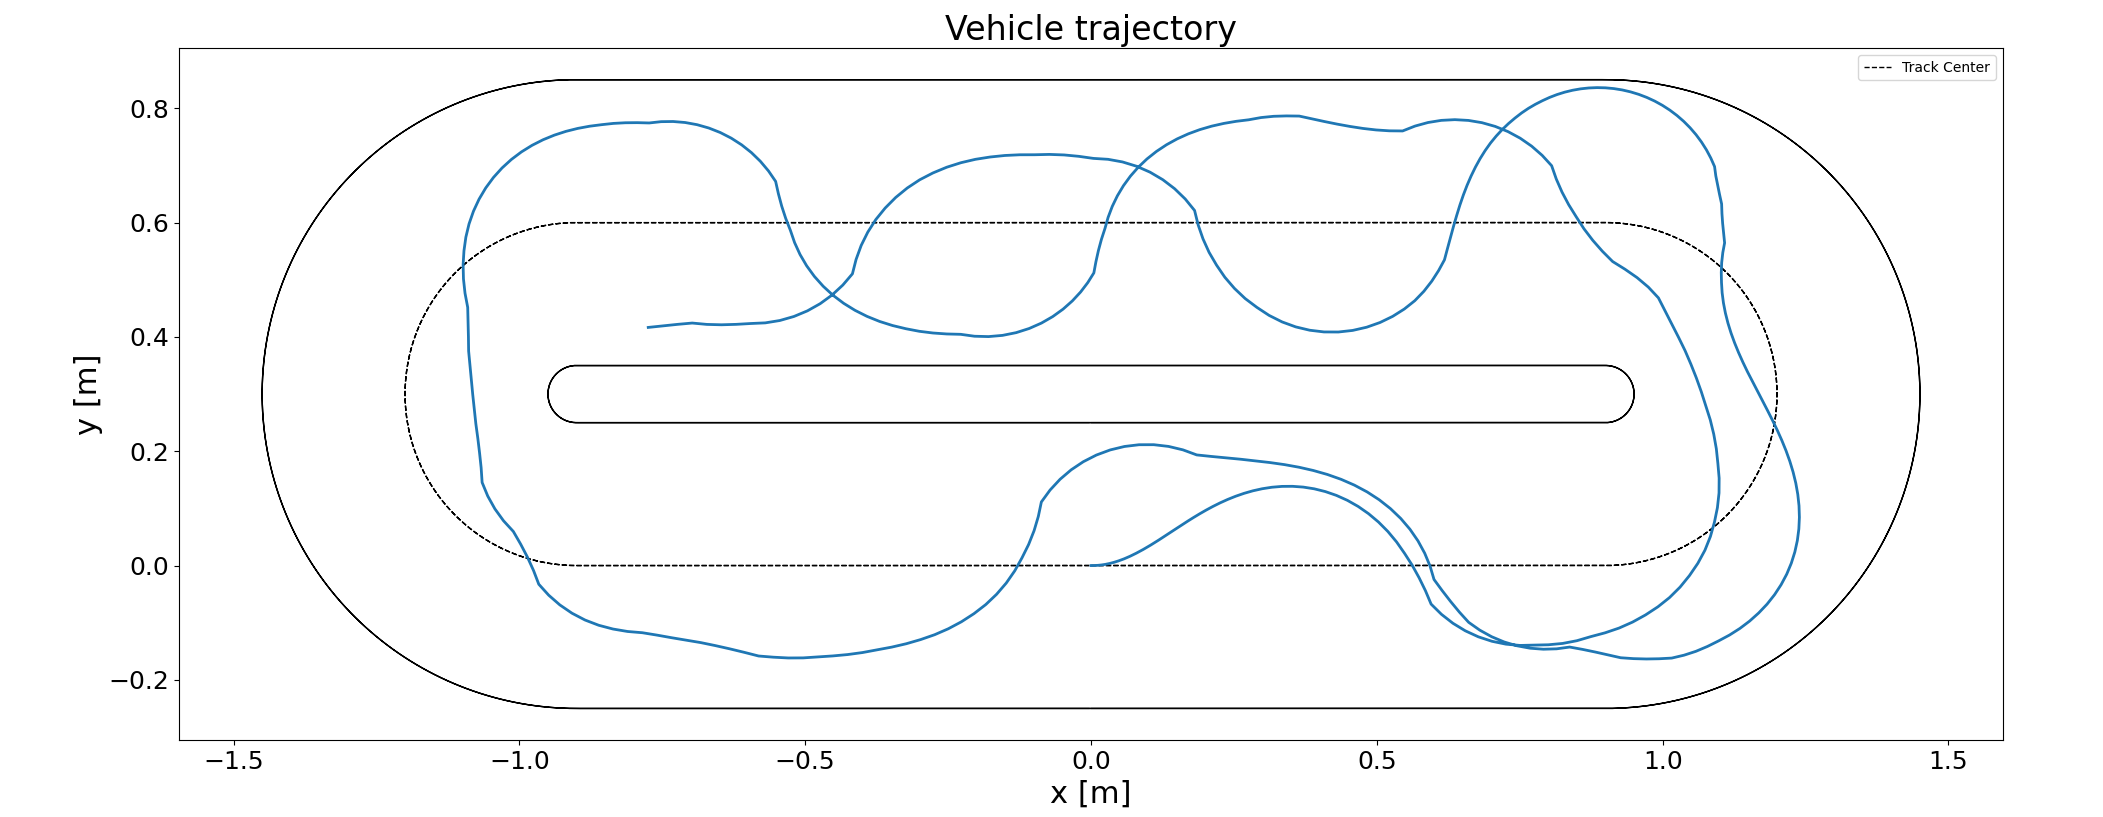
\includegraphics[width=0.9\textwidth]{\imagedir/kinematic-trajectory.png}
    \caption{Path of the vehicle, the dotted line being the track centerline and the blue line being the path}
    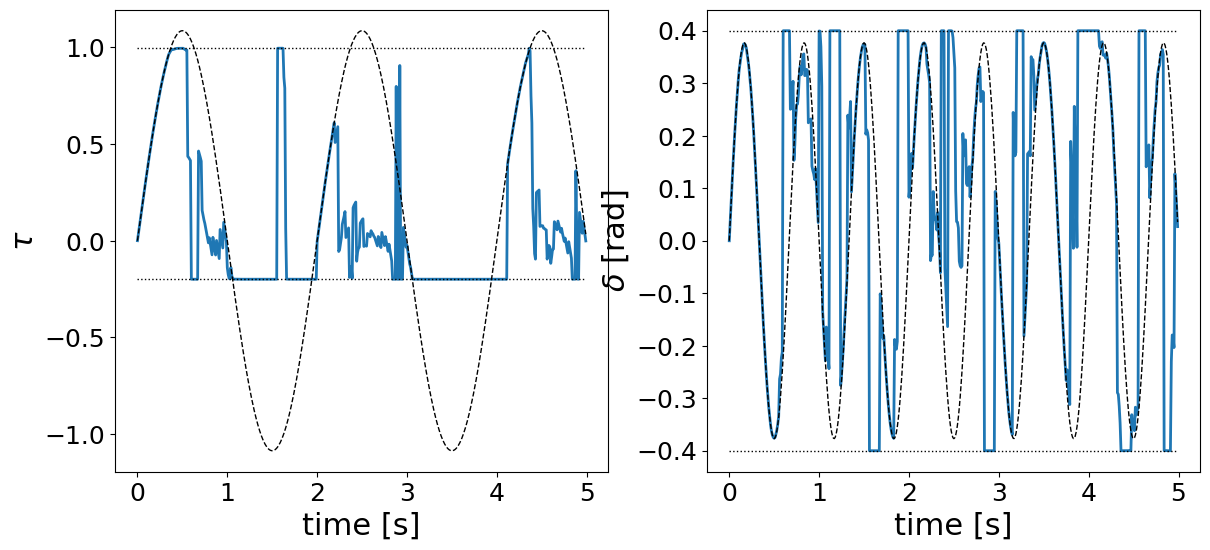
\includegraphics[width=0.9\textwidth]{\imagedir/kinematic-sin-sin-inputs.png}
    \caption{Objective and applied inputs, the dotted line being the objective input and blue line being the applied input}
    \label{fig:kinematic-single-run}
\end{figure}

We can see from \cref{fig:kinematic-single-run}, the objective inputs are modified by the safety filter and it successfully keeps the vehicle on the track.

We also present the result of applying different terminal ingredients, as mentioned in \cref{sec:design-terminal-ingredient}.
Here the objective input is set to full throttle $\tau_s = \tau_{\max}$.
The hyperparameters are adjusted for each terminal ingredient.
To avoid the hyperparameters to overfit to this specific objective control, they are tuned so to make sure that the vehicle can successfully drive around the track with three different objective control input rules, including `Max Throttle with Zero Steering', `Max Throttle with Sine Steering' and `Sine Throttle with Sine Steering'.

\begin{figure}[ht]
    \centering
    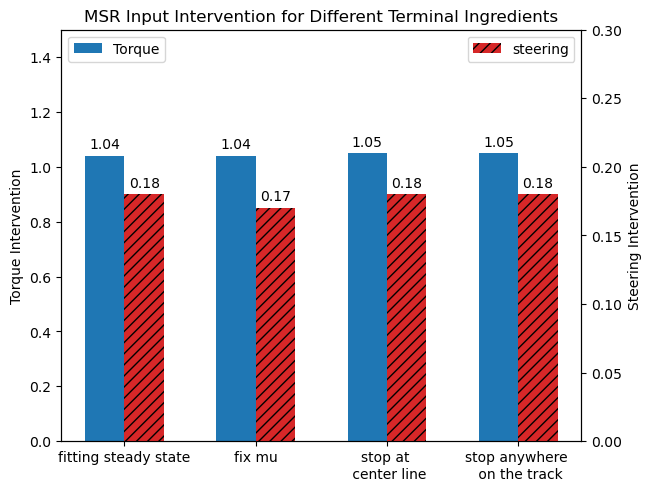
\includegraphics[width=0.7\textwidth]{\imagedir/kinematic-terminal-comparison.png}
    \caption{Input interference for different terminal ingredients}
    \label{fig:kinematic-terminal-comparison}
\end{figure}

We can see from \cref{fig:kinematic-terminal-comparison} that, with finely tuned hyperparameters, all the terminal ingredients have very similar mean squared input interference.

It's worth noting that, it's not necessary true that smaller mean squared input interference means better performance for a safety filter.
For example, a safety filter can have smaller mean squared input interference by always modifying the input to some point, so the vehicle can always stay near the centerline.
While another safety filter will only make large interference when the vehicle is about to leave the track, resulting in a larger mean square input interference.
However, the second safety filter is more desirable, as it will not interfere with the vehicle when it is driving normally.
There are no good metrics to evaluate the performance of a safety filter yet, and we will not discuss this topic further in this Thesis.


\section{Simulation Using Dynamic Model}\label{sec:result-dynamic-model}

This section presents the result for the safety filter on the dynamic model.
As stated before, we only use the ``Fixing $\mu$ and Velocity in Optimization Problem'' method to find the terminal ingredient.

Also, we assume we have noise-free access to the output, both in the dataset and online observation.
We take use of the prediction method introduced in \cref{chap:non-linear-system} to make predictions for the dynamic model.
The prediction horizon is set to $L=80$, number of input-output pairs used for initial condition set to $l=10$, and the constraint tightening constants being: $[0.25, 0.1, 0.05, 0.01] \times \elat_{\max}$, $[0.2, 0.1, 0.05, 0.01] \times \mu_{\max}$, $[0.2, 0.1, 0.05, 0.01] \times \vx_{\max}$, and $[0.1, 0.05, 0.01, 0.005] \times \vy_{\max}$, for the corresponding four outputs.
For the prediction method, we choose $Q$ so that all the input/outputs are normalized by the corresponding maximum value, and the weighting function $w(d) = \frac{1}{d}$.
Similar to the case in \cref{sec:non-linear-system-numerical-example}, we only use the trajectory slices that are close enough to current initial state, if enough number of such slices are available.

Before the simulation, a dataset trajectory of length $N=1000$ is collected, by a similar method in \cref{sec:result-kinematic-model}.
In addition, we introduce a scheme of collecting more dataset with a more realistic method, as can be seen in \cref{fig:data-collection-process}.

\includefig{data-collection-process.png}{0.7}{The process of dataset collection, each run uses a different controller or objective input scheme, and stops after safe constraint not satisfied}{fig:data-collection-process}

In this framework, in addition to the dataset collected by the method in \cref{sec:result-kinematic-model}, we also collect online-data starting from a realistic initial condition and realistic objective input, which does not use knowledge of the system parameters.
Here in the dataset collection runs, we set the objective input to be a sine wave with randomly chosen frequency and phase.
As can be seen from \cref{fig:data-collection-process}, At each iteration a data-collection process is conducted, and the dataset is updated.
After that, in application runs, the new dataset is used for the safety filter.
We do not directly use dataset from the application runs, to avoid the weighting method putting too much weight onto several trajectory slices that are very close to current state.
This can be a problem, when at each iteration the same controller or objective input is applied, as the system will travel along a very similar trajectory.
For this certain example, in the application runs, we apply three different kinds of open loop objective input, as introduced in \cref{sec:result-kinematic-model}.

As the final result, after two iterations, the safety filter is able to keep the vehicle within the track boundaries for all application runs.
Here we present the trajectory and inputs with the objective input being `Sine Throttle with Sine Steering', as can be seen in \cref{fig:dynamic-single-run}.


\begin{figure}[ht]
    \centering
    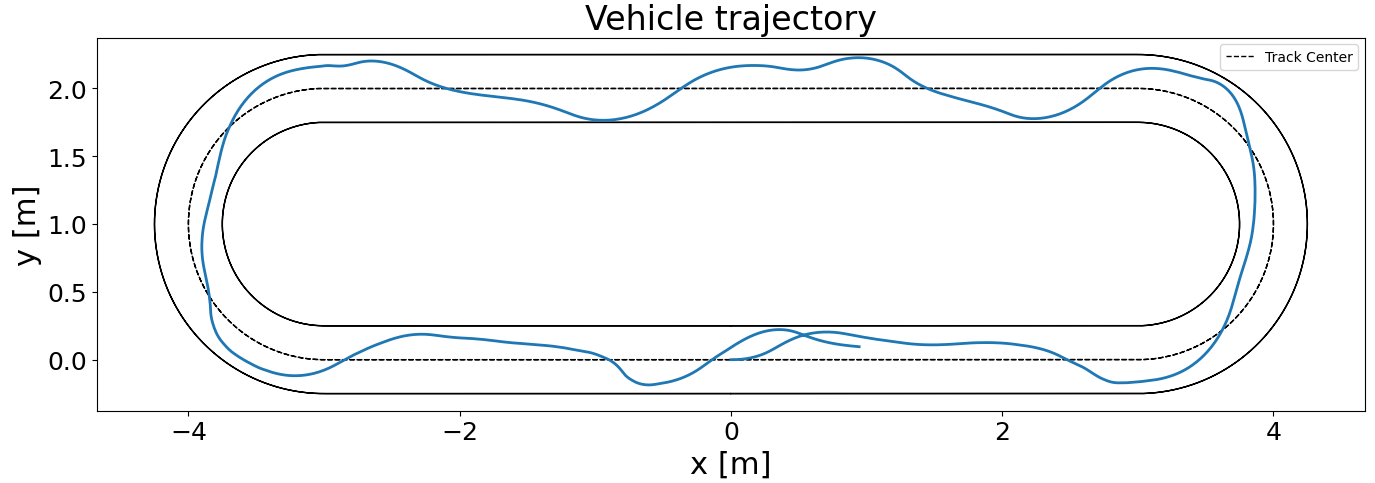
\includegraphics[width=0.9\textwidth]{\imagedir/dynamic-sin-sin-trajectory.png}
    \caption{Path of the vehicle, the dotted line being the track centerline and the blue line being the path}
    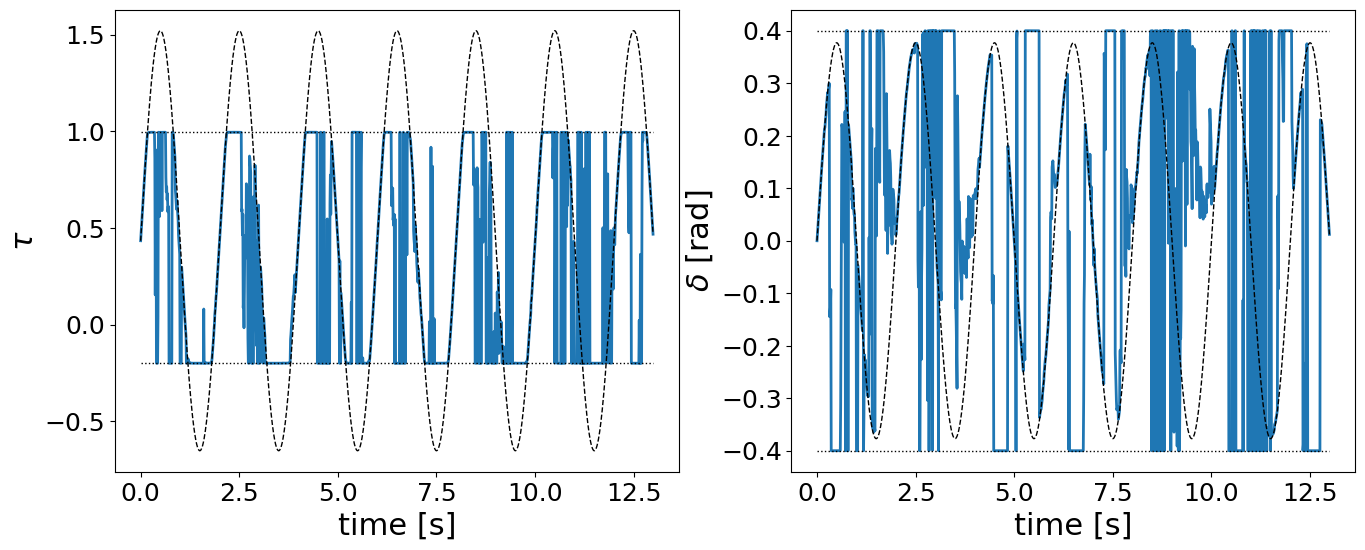
\includegraphics[width=0.9\textwidth]{\imagedir/dynamic-sin-sin-inputs.png}
    \caption{Objective and applied inputs, the dotted line being the objective input and blue line being the applied input}
    \label{fig:dynamic-single-run}
\end{figure}

We can see from \cref{fig:dynamic-single-run}, the safety filter is able to keep the vehicle within the track boundaries, even with the more realistic dynamic model.
There are still many improvements to be made for the safety filter, though.
For example, the resulting input sequence is not smooth, and can not be applied to the real RC vehicle.
Also, similar improvements mentioned for the prediction method in \cref{sec:weighting-method} can also be applied to the safety filter.

\cleardoublepage
\chapter{Conclusion and Future Work}\label{chap:conclusion}

In this thesis, we proposed different formulations of data-driven predictive safety filter, data-driven prediction method for non-linear systems, a metric to estimate the richness of datasets of non-linear systems, and applied the data-driven predictive safety filter to the model of a miniature racing vehicle.

The filter for noise-free LTI systems is designed in \cref{chap:nominal-ddsf}, and it is proven that it is equivalent to the model-based predictive safety filter.

For noisy LTI systems, we proposed two different robust data-driven predictive safety filters in \cref{chap:robust-ddsf-lti}, namely the direct and indirect robust data-driven predictive safety filters.
They both have similar qualitative guarantees, but numerical results show that the indirect robust data-driven predictive safety filter is less conservative than the direct robust data-driven predictive safety filter and yields better performance.
A more rigorous and systematic way of choosing the hyperparameters, especially the constraint tightening constants, is left for future work.

In \cref{chap:non-linear-system}, we proposed a data-driven method to make predictions for nonlinear systems.
We also proposed a metric based on fractal dimension to estimate the richness of datasets of nonlinear systems.
By a numerical example of two-dimensional nonlinear system, we showed that with properly chosen hyperparameters, the proposed prediction method yields more precise prediction than existing methods.
Also, the metric is higher for richer datasets.
There are many directions for further research in this area.
For example, hyperparameters used in the weighting scheme can vary according to the extended state.
It will also be interesting to find a systematic way of optimizing these hyperparameters, probably by using machine learning techniques.
It is also possible to incorporate the weighting method into the direct method.
By using the metric to estimate the richness of datasets, we can also try to construct richer datasets with shorter trajectories.

In \cref{chap:test-chronos}, we applied the indirect robust data-driven predictive safety filter and the proposed prediction method to the model of a miniature racing vehicle.
We showed that with the simplified kinematic model, the filter is able to keep the vehicle within track boundaries, even with practical level of noise.
Different forms of terminal constraints for the vehicle model are also proposed and compared.
For the dynamic model, with the prediction method introduced in \cref{chap:non-linear-system} and noise-free observation, the filter is also able to keep the vehicle within track boundaries.
It is still not clear how to systematically evaluate the overall performance of a safety filter, and some improvements will be needed before the filter can be applied to a real RC vehicle.


% \chapter{Introduction}\label{sec:introduction}
This template is meant to be used for semester, bachelor, and master theses written at the Institute for Dynamic Systems and Control (IDSC), ETH Zurich. The template includes several examples of equations, figures, tables, etc. in order to act as a {\it very} short introduction to \TeX\! and \LaTeX. Yet, the template is also provided to ensure that all written work at IDSC shares identical formatting.

\section{The Preamble}\label{sec:preamble}
The preamble of the \LaTeX\! template defines the font size, page layout, language, report type, title, and author(s) of the report. The preamble of the current template is shown below. It should be more or less clear how you need to modify the preamble to fit your needs; if not, consult your supervisor.
%\lstset{language=TeX,numbers=none}
%\begin{lstlisting}[frame=lines]
\begin{verbatim}
 \documentclass[10pt,twoside,a4paper,fleqn]{report}

 \usepackage[german,st]{ethidsc}             % IDSC style
                                             % {german}/english: language
                                             % {st}/bt/mt: thesis type

 % Page header (don't change)
 \setlength{\parindent}{0em}                 % Disable parindent
 \rhead[\nouppercase{\rightmark}]{\thepage}  % Special headings
 \lhead[\thepage]{\nouppercase{\leftmark}}   % Special headings
 \cfoot{}                                    % Special headings

 % Title page (please fill in)
 \title{\LaTeX\ Thesis Template v.1.4}       % Report title

 \studentA{Hans Muster}
 \ethidA{97-906-739}
 \semesterA{5}
 \emailA{muster@student.ethz.ch}

 % \studentB{Second Student}
 % \ethidB{12-345-678}
 % \semesterB{9}
 % \emailB{second@student.ethz.ch}

 \supervision{First Supervisor\\ Prof. Dr. Second Supervisor}
 \date{March 2011}

 \identification{IDSC-XX-YY-ZZ}              % Project identifier

 \infopage
 \declaration
 \end{verbatim}
%\end{lstlisting}

The style \texttt{ethidsc.sty} enforces certain changes to the original \texttt{report} class, e.g., the title page. The style accepts two options. The first option lets you choose the language of your report, i.e., the language of the title page, headings, info-page, etc. Valid options are: \texttt{german} (default) and \texttt{english}. The second option defines the type of report which will be printed on the title and info page. Valid options are: \texttt{st} (default), \texttt{bt}, and \texttt{mt} for semester, bachelor and master thesis, respectively. For instance, if you will be writing a master thesis in English, use
\begin{verbatim}
 \usepackage[english,mt]{ethidsc}
\end{verbatim}
The command \texttt{\textbackslash infopage} prints an information page at the end of the document which you must sign before handing in the report.


% \cleardoublepage
% \chapter{Working with \LaTeX\ }\label{sec:working}
This chapter explains how to typeset some of the most common elements contained in a technical report using \LaTeX.

\section{Headings}
Your report can be structured using several different types of headings. Use the commands \texttt{\textbackslash chapter\{.\}}, \texttt{\textbackslash section\{.\}}, \texttt{\textbackslash subsection\{.\}}, and \texttt{\textbackslash subsubsection\{.\}}. Use the asterisk symbol \texttt{*} to suppress numbering of a certain heading if necessary, for example, \texttt{\textbackslash section*\{.\}}.

\section{References and Footnotes}\label{sec:references}
References to literature are included using the command \texttt{\textbackslash
cite\{.\}}. For example \cite{optreg,motsys}. Your references must be entered in the file \texttt{bibliography.bib}. Making changes or adding new references in the bibliography file can be done manually or by using specialized software such as \textit{JabRef} which is free of charge.
 
Cross-referencing within the text is easily done using \texttt{\textbackslash label\{.\}} and \texttt{\textbackslash ref\{.\}}. For example, this paragraph is part of chapter~\ref{sec:working}; more specifically section~\ref{sec:references} on page~\pageref{sec:references}. You will need to compile your document twice in order for the cross-referencing to be updated.

Footnotes\footnote{The use of footnotes is generally not recommended.} are added using the command \texttt{\textbackslash footnote\{.\}}, but try to avoid the used of footnotes altogether.

\section{Lists}\label{sec:lists}
Three types of list-environments are commonly used: \texttt{itemize}, \texttt{enumerate}, and \texttt{description}. The following example uses \texttt{itemize} to create a list without numbering
\begin{itemize}
  \item point one; and
  \item point two
\end{itemize}
created using
\begin{verbatim}
\begin{itemize}
  \item point one; and
  \item point two
\end{itemize}
\end{verbatim}

The following example uses \texttt{enumerate} to create a list with numbering
\begin{enumerate}
  \item point one; and
  \item point two
\end{enumerate}
created using
\begin{verbatim}
\begin{enumerate}
  \item point one; and
  \item point two
\end{enumerate}
\end{verbatim}

The following example uses \texttt{description} to create a list with custom text as bullet-points
\begin{description}
  \item[P1] point one; and
  \item[P2] point two
\end{description}
created using
\begin{verbatim}
\begin{description}
  \item[P1] point one; and
  \item[P2] point two
\end{description}
\end{verbatim}


\section{Tables}\label{sec:tables}
Table~\ref{tab:table} shows an example of a simple table-layout. Try to avoid vertical lines on tables. The Internet contains countless resources on how to create special elements and structures in tables such as cells spanning multiple rows, rotated text, sideways tables, justification of cell elements, etc.
\begin{table}[ht]
\begin{center}
\caption{Driving cycle data of ECE-15, EUDC, and NEDC.}\vspace{1ex}
\label{tab:table}
\begin{tabular}{llccc}\hline
Description & Unit & ECE & EUDC & NEDC \\ \hline
Duration & s & 780 & 400 & 1180 \\
Distance & km & 4.052 & 6.955 & 11.007 \\
Average velocity & km/h & 18.7 &  62.6 & 33.6 \\
Idle speed & \% & 36 & 10 & 27 \\ \hline
\end{tabular}
\end{center}
\end{table}

This table was created using
\begin{verbatim}
\begin{table}[ht]
\begin{center}
\caption{Driving cycle data of ECE-15, EUDC, and NEDC.}\vspace{1ex}
\label{tab:table}
\begin{tabular}{llccc}\hline
Description & Unit & ECE & EUDC & NEDC \\ \hline
Duration & s & 780 & 400 & 1180 \\
Distance & km & 4.052 & 6.955 & 11.007 \\
Average velocity & km/h & 18.7 &  62.6 & 33.6 \\
Idle speed & \% & 36 & 10 & 27 \\ \hline
\end{tabular}
\end{center}
\end{table}
\end{verbatim}
Table~\ref{tab:table_advanced} shows a more advanced version of Tab.~\ref{tab:table} using the \texttt{booktabs} package. Inspect the source code of this document to see how this was done.
\begin{table}[ht]
\begin{center}
\small
\caption{Driving cycle data of ECE-15, EUDC, and NEDC.}\vspace{1ex}
\label{tab:table_advanced}
\begin{tabular}{@{}lcccc@{}}\toprule[1.5pt]
& & \multicolumn{3}{c}{\bf Driving cycle}\\
\cmidrule{3-5}
Description & Unit & {ECE} & {EUDC} & {NEDC} \\ \midrule
Duration & \unit[]{s} & 780 & 400 & 1180 \\
Distance & \unit[]{km} & 4.052 & 6.955 & 11.007 \\
Average velocity & \unitfrac[]{km}{h} & 18.7 &  62.6 & 33.6 \\
Idle speed & \unit[]{\%} & 36 & 10 & 27 \\ \bottomrule[1.5pt]
\end{tabular}
\end{center}
\end{table}



\section{Working with Units}
The package \texttt{\textbackslash usepackage\{units\}} enables two useful commands, namely \texttt{\textbackslash unit[.]\{.\}} and \\ \texttt{\textbackslash unitfrac[.]\{.\}\{.\}}. Use these commands to display units in a concise way, for example
\begin{align}
\delta t &= \unit[1]{s}\\
v &= \unitfrac[5]{m}{s}.
\end{align}
This example was done using
\begin{verbatim}
\begin{align}
\delta t &= \unit[1]{s}\\
v &= \unitfrac[5]{m}{s}.
\end{align}
\end{verbatim}

\section{Including Graphics}\label{sec:epsgraph}
It is recommended that you only use encapsulated post-script graphics \texttt{.eps} in your report. If you mix \texttt{.eps} with other formats such as \texttt{.png}, \texttt{.jpeg} or \texttt{.gif}, you will most likely not be able to compile your report without errors. Note that figures created in \textsc{Matlab} are easily saved in \texttt{.eps} format.

The inclusion of a figure can be done in the following way:
\begin{verbatim}
\begin{figure}[ht]
   \centering
   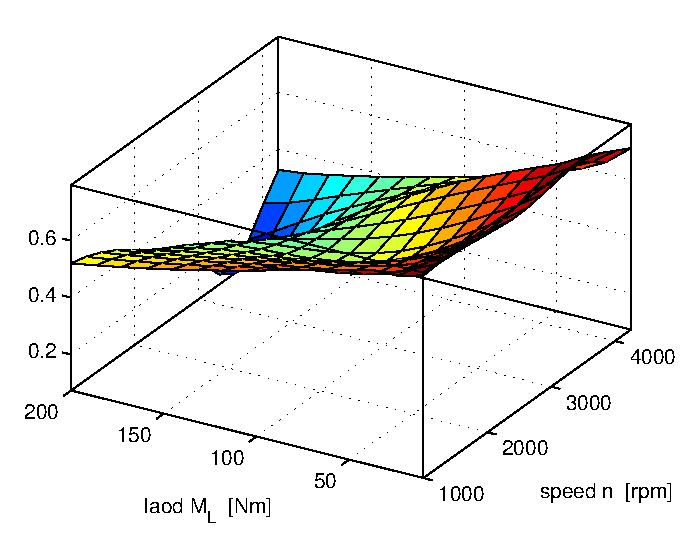
\includegraphics[width=0.75\textwidth]{img/k_surf.eps}
   \caption{Example of a figure.}
   \label{img:k_surf}
\end{figure}
\end{verbatim}

\begin{figure}[ht]
   \centering
   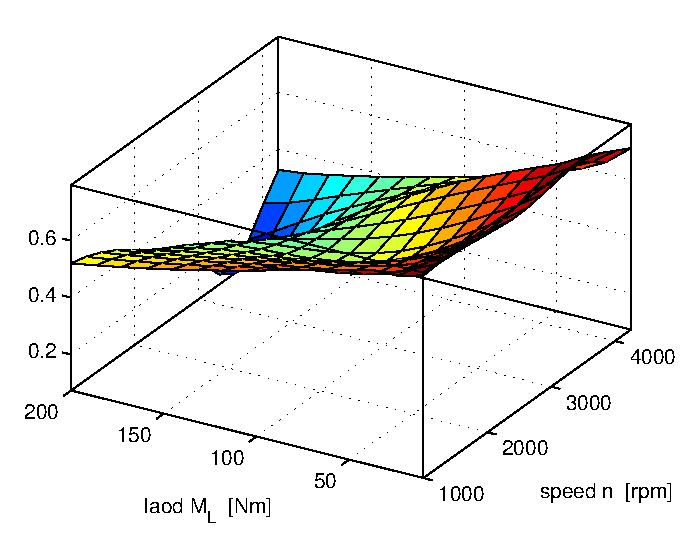
\includegraphics[width=0.75\textwidth]{img/k_surf.eps}
   \caption{Example of a figure.}
   \label{img:k_surf}
\end{figure}

Two figures are displayed next to each other using
\begin{verbatim}
\begin{figure}[ht]
  \begin{minipage}[t]{0.48\textwidth}
    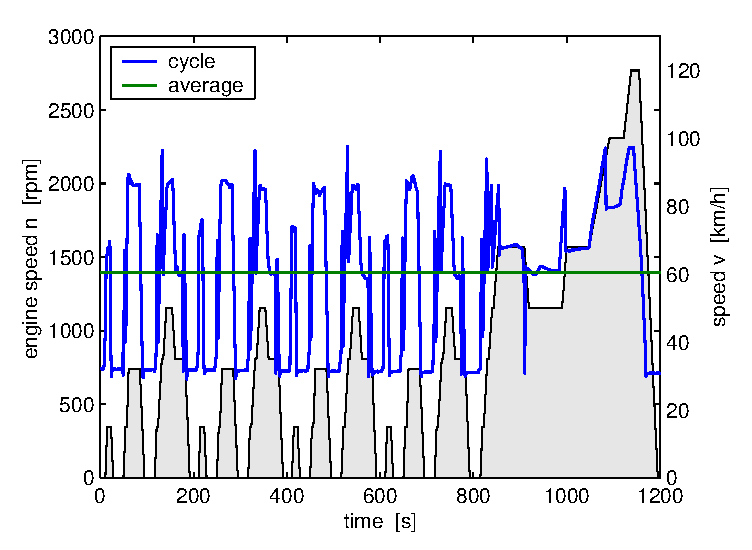
\includegraphics[width = \textwidth]{img/cycle_we.eps}
  \end{minipage}
  \hfill
  \begin{minipage}[t]{0.48\textwidth}
    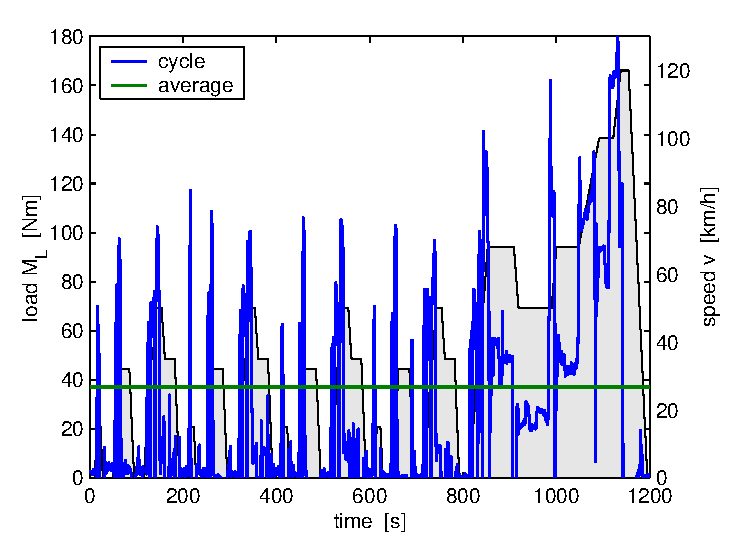
\includegraphics[width = \textwidth]{img/cycle_ml.eps}
  \end{minipage}
  \caption{Two figures next to each other.}
  \label{img:cycle}
\end{figure}
\end{verbatim}

\begin{figure}[ht]
  \begin{minipage}[t]{0.48\textwidth}
    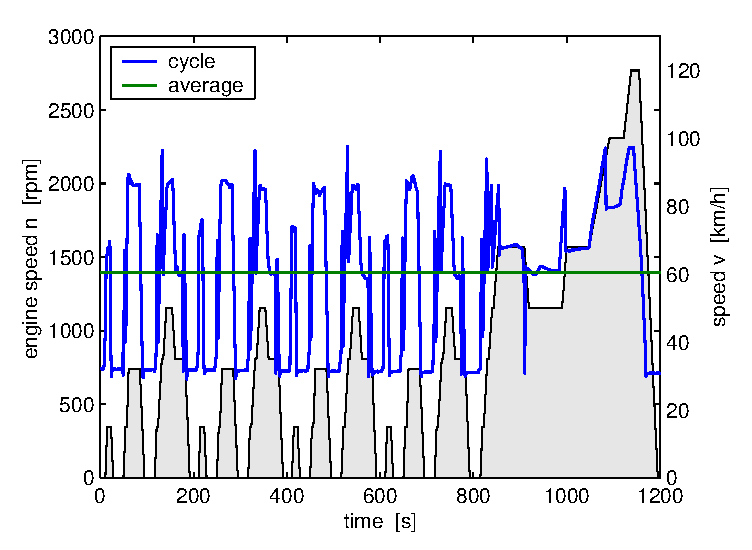
\includegraphics[width = \textwidth]{img/cycle_we.eps}
  \end{minipage}
  \hfill
  \begin{minipage}[t]{0.48\textwidth}
    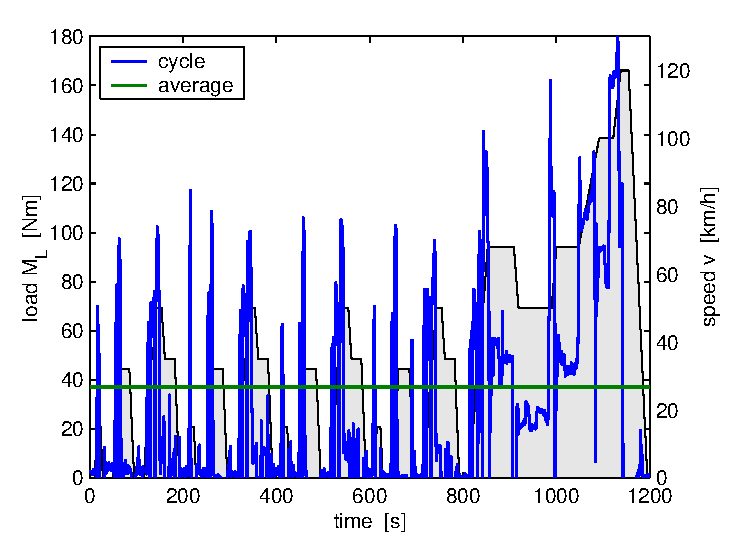
\includegraphics[width = \textwidth]{img/cycle_ml.eps}
  \end{minipage}
  \caption{Two figures next to each other.}
  \label{img:cycle}
\end{figure}

The positioning parameter \texttt{h} (here) forces your figure to be placed in the current position relative to your text. You may add \texttt{t} (top), \texttt{b} (bottom), and/or \texttt{p} (page) to allow for more flexible positioning within your document. For instance, \texttt{[tb]} forces your figure to be placed either on the top or bottom of a page.


\section{Equations}\label{sec:math}
The most common way to include equations is using the \texttt{equation} environment.
\begin{equation}\label{eq:p_me0f}
 p_\mathrm{me0f}(T_e,\omega_e) \ = \ k_1(T_e) \cdot (k_2+k_3 S^2
 \omega_e^2) \cdot \Pi_\mathrm{max} \cdot \sqrt{\frac{k_4}{B}} \, .
\end{equation}
It is recommended to use \texttt{\textbackslash mathrm\{.\}} for subscripts comprising more than two letters since it reduces the width of the subscript significantly and improves readability. The corresponding code is
\begin{verbatim}
\begin{equation}\label{eq:p_me0f}
 p_\mathrm{me0f}(T_e,\omega_e) \ = \ k_1(T_e) \cdot (k_2+k_3 S^2
 \omega_e^2) \cdot \Pi_\mathrm{max} \cdot \sqrt{\frac{k_4}{B}} \, .
\end{equation}
\end{verbatim}
Equations, such as Eq.~\eqref{eq:p_me0f}, may be referenced using \texttt{\textbackslash eqref\{.\}}. In-line mathematical content is created using \texttt{\$.\$}, for example $a^2+b^2=c^2$. It is practically possible to typeset any equation in \LaTeX. Equation~\eqref{eq:advanced} shows an example of a more advance structure.
\begin{equation}\label{eq:advanced}
x^k_n(i) = \left\{\begin{array}{ll}y(i) & \text{if}\quad x^k_{n-1}(i)\leq \mathbf{x}\\
z(i) & \text{otherwise}\end{array}\right., \text{for}\quad i=\{1,\ldots,N\}.
\end{equation}



\section{Including Code in your Document}
Include samples from your Matlab code using the \texttt{lstlistings} environment, for example
\lstset{language=Matlab,numbers=none}
\begin{lstlisting}[frame=lines]
% Evaluate y = 2x
for i = 1:length(x)

  y(i) = 2*x(i);

end
\end{lstlisting}
This example was created using
\begin{verbatim}
\lstset{language=Matlab,numbers=none}
\begin{lstlisting}[frame=lines]
% Evaluate y = 2x
for i = 1:length(x)

  y(i) = 2*x(i);

end
\end{lstlisting}
\end{verbatim}
where \texttt{\textbackslash usepackage\{mcode\}} must be included in the preamble of your document. If you want to include the entire content of a file \texttt{mycode.m} in your document, simply input the path to \texttt{mycode.m} instead of pasting the entire content into your \TeX -file
\begin{verbatim}
\lstset{language=Matlab,numbers=left}
\lstinputlisting{path/to/mycode.m}
\end{verbatim}
Including the path to your m-file also ensures that the code in your report is always up-to-date. The \texttt{\textbackslash lstset\{language=Matlab\}} command ensures that \textsc{Matlab} syntax definitions are used, but many other languages are recognised as well such as \texttt{Fortran} and \texttt{C++}.

% \cleardoublepage
% \input{}
% \cleardoublepage
% \input{}
% \cleardoublepage
% ...

% Appendix______________________________________________________________________
\appendix
\chapter{Something}\label{sec:something}

Blah, blah \dots

 \cleardoublepage


\chapter{Again Something}\label{sec:again_something}

Blah, blah again. \dots

 \cleardoublepage



% Bibliography__________________________________________________________________
% Literature (Additional references can be added to the .bib-file manually, or by using, for example, the free application JabRef). Compile in the following order: latex -bibtex -latex -latex

\bibliographystyle{ieeetr}
\bibliography{bibliography}

\end{document}
